% Arquivo LaTeX de exemplo de dissertação/tese a ser apresentados à CPG do IME-USP
% 
% Versão 5: Sex Mar  9 18:05:40 BRT 2012
%
% Criação: Jesús P. Mena-Chalco
% Revisão: Fabio Kon e Paulo Feofiloff
%  
% Obs: Leia previamente o texto do arquivo README.txt

\documentclass[12pt,twoside,a4paper]{book}

% ------------------------------------------------------------------- %
% pacotes 


\usepackage{adjustbox}
\usepackage{graphicx}
\usepackage[hyphens,obeyspaces,spaces]{url}
\usepackage[T1]{fontenc} 
\usepackage[portuguese]{babel}
\usepackage[utf8]{inputenc}
\usepackage{float}
\usepackage{amsmath}
\usepackage{amsthm}
\usepackage{amsfonts}
\usepackage{algpseudocode}
\usepackage{amssymb}
\usepackage[pdftex]{graphicx}           % usamos arquivos pdf/png como figuras
\usepackage{setspace}                   % espaçamento flexível
\usepackage{indentfirst}                % indentação do primeiro parágrafo
\usepackage{makeidx}                    % índice remissivo
\usepackage[nottoc]{tocbibind}          % acrescentamos a bibliografia/indice/conteudo no Table of Contents
\usepackage{courier}                    % usa o Adobe Courier no lugar de Computer Modern Typewriter
\usepackage{type1cm}                    % fontes realmente escaláveis
\usepackage{listings}                   % para formatar código-fonte (ex. em Java)
\usepackage{titletoc}
\usepackage[fixlanguage]{babelbib}
\usepackage[font=small,format=plain,labelfont=bf,up,textfont=it,up]{caption}
\usepackage[usenames,svgnames,dvipsnames]{xcolor}
\usepackage[a4paper,top=3.0cm,bottom=2.0cm,left=3.0cm,right=2.0cm]{geometry} % margens
\usepackage[pdftex,plainpages=false,pdfpagelabels,pagebackref,colorlinks=true,citecolor=DarkGreen,linkcolor=NavyBlue,urlcolor=DarkRed,filecolor=green,bookmarksopen=true]{hyperref} % links coloridos
\usepackage[all]{hypcap} % soluciona o problema com o hyperref e capitulos
\usepackage[round,sort,nonamebreak]{natbib} % citação bibliográfica textual(plainnat-ime.bst)

% \usepackage{algorithm}
% \usepackage{mathtools}
% \usepackage[noend]{algpseudocode}

\fontsize{60}{62}\usefont{OT1}{cmr}{m}{n}{\selectfont}

% ------------------------------------------------------------------- %
% Cabeçalhos similares ao TAOCP de Donald E. Knuth
\usepackage{fancyhdr}
\pagestyle{fancy}
\fancyhf{}
\renewcommand{\chaptermark}[1]{\markboth{\MakeUppercase{#1}}{}}
\renewcommand{\sectionmark}[1]{\markright{\MakeUppercase{#1}}{}}
\renewcommand{\headrulewidth}{0pt}

\allowdisplaybreaks

% ------------------------------------------------------------------- %
\graphicspath{{./figuras/}}             % caminho das figuras (recomendável)
\frenchspacing                          % arruma o espaço: id est (i.e.) e exempli gratia (e.g.) 
\urlstyle{same}                         % URL com o mesmo estilo do texto e não mono-spaced
\makeindex                              % para o índice remissivo
\raggedbottom                           % para não permitir espaços extra no texto
\fontsize{60}{62}\usefont{OT1}{cmr}{m}{n}{\selectfont}
\cleardoublepage
\normalsize

% ------------------------------------------------------------------- %
% Opções de listing usados para o código fonte
% Ref: http://en.wikibooks.org/wiki/LaTeX/Packages/Listings
\lstset{
    basicstyle=\ttfamily,           % the size of the fonts that are used for the code
    stepnumber=1,                   % the step between two line-numbers. If it's 1 each line will be numbered
    showspaces=false,               % show spaces adding particular underscores
    showstringspaces=false,         % underline spaces within strings
    showtabs=false,                 % show tabs within strings adding particular underscores
    framerule=0.6pt,
    tabsize=2,                      % sets default tabsize to 2 spaces
    captionpos=b,                   % sets the caption-position to bottom
    breaklines=true,                % sets automatic line breaking
    breakatwhitespace=false,        % sets if automatic breaks should only happen at whitespace
    frame=single,                   % adds a frame around the code
    rulecolor=\color{gray},         % if not set, the frame-color may be changed on line-breaks within not-black text (e.g. comments (green here))
    extendedchars=true,
    xleftmargin=10pt,
    xrightmargin=10pt,
    framexleftmargin=10pt,
    framexrightmargin=10pt
}

% Comandos customizados
\newcommand{\diag}{\operatorname{diag}}
\newcommand{\yi}{{\boldsymbol{y}_{(i)}}}
\newcommand{\bhat}{{\hat{\boldsymbol{\beta}}}}
\newcommand{\sigsq}{\sigma^2}
\newcommand{\tausq}{{\tau^2}}
\newcommand{\ubf}{{\boldsymbol{u}}}
\newcommand{\vbf}{{\boldsymbol{v}}}
\newcommand{\tbf}{{\boldsymbol{t}}}
\newcommand{\ybf}{{\boldsymbol{y}}}
\newcommand{\transp}{{\mathsf{T}}}
\newcommand{\betabf}{{\boldsymbol{\beta}}}
\newtheorem{thm}{Teorema}
\newtheorem{prop}{Proposição}[chapter]
% ------------------------------------------------------------------- %
% Corpo do texto
\begin{document}
\frontmatter 
% cabeçalho para as páginas das seções anteriores ao capítulo 1 (frontmatter)
\fancyhead[RO]{{\footnotesize\rightmark}\hspace{2em}\thepage}
\setcounter{tocdepth}{2}
\fancyhead[LE]{\thepage\hspace{2em}\footnotesize{\leftmark}}
\fancyhead[RE,LO]{}
\fancyhead[RO]{{\footnotesize\rightmark}\hspace{2em}\thepage}
\onehalfspacing  % espaçamento

% ------------------------------------------------------------------- %
% CAPA
% Nota: O título para as dissertações/teses do IME-USP devem caber em um 
% orifício de 10,7cm de largura x 6,0cm de altura que há na capa fornecida pela SPG.
\thispagestyle{empty}
\begin{center}
    \vspace*{2.3cm}
    
    \Large{\textbf{Predição de polaridade negativa\\
    em relatórios de auditoria\\
    utilizando dados socioeconômicos}}
    
    \vspace*{1.2cm}
    \Large{Lucas Peinado Bruscato}
    
    \vskip 2cm
    \textsc{
    Dissertação apresentada\\[-0.25cm] 
    ao\\[-0.25cm]
    Instituto de Matemática e Estatística\\[-0.25cm]
    da\\[-0.25cm]
    Universidade de São Paulo\\[-0.25cm]
    para\\[-0.25cm]
    obtenção do título\\[-0.25cm]
    de\\[-0.25cm]
    Mestre em Ciências}
    
    \vskip 1.5cm
    Programa: Estatística\\
    Orientador: Profa. Dra. Florencia Leonardi

    \vskip 1cm
    \normalsize{}
    
    \vskip 0.5cm
    \normalsize{São Paulo, fevereiro de 2020}
\end{center}


\newpage
\thispagestyle{empty}
\begin{center}
    \vspace*{2.3 cm}
    
    \textbf{\Large{Predição de polaridade negativa\\
    em relatórios de auditoria\\
    utilizando dados socioeconômicos}}\\
    
    \vspace*{2 cm}
\end{center}

\vskip 2cm

\begin{flushright}
    Esta é a versão original da dissertação/tese elaborada pelo\\
    candidato Lucas Peinado Bruscato, tal como\\
    submetida à Comissão Julgadora.
    
    \vskip 2cm

\end{flushright}

\vskip 4.2cm

% ------------------------------------------------------------------- %
% Agradecimentos:
% Se o candidato não quer fazer agradecimentos, deve simplesmente eliminar esta página 
\chapter*{Agradecimentos}

À minha mãe Helena Peinado Viotto e ao meu pai Tadeu Henrique Bruscato que não mediram esforços, em toda a vida, para que eu pudesse chegar onde cheguei, ser o que sou. Minha mãe pela persistência e meu pai pela inspiração à curiosidade. São e sempre serão meus exemplos a serem seguidos na vida.

À minha esposa e melhor amiga Natália de Deus Vilela pelo companheirismo e compreensão nesse último passo do mestrado que foi intenso e extenso, ainda mais sendo realizado em nosso novo país de residência.

À minha orientadora Florencia Leonardi pela paciência, orientação e todo conhecimento transferido nestes anos de trabalho. O apoio em realizar um trabalho com um tema considerado incomum no programa foi de uma grandeza imensurável.

Aos amigos Rachel Ubriaco por realizar críticas construtivas sobre o trabalho, Diego Wesllen por me motivar desde o primeiro momento a realizar a disciplina de Probabilidade e Inferência I e Bruno Carvalho pelas discussões técnicas que me motivaram na realização deste trabalho.

Ao Instituto de Matemática e Estatística da Universidade de São Paulo e todos os seus professores, em especial os do departamento de estatí́stica, por fazerem parte da minha formação em estatística.

\pagenumbering{roman}

% ------------------------------------------------------------------- %
% Resumo
\chapter*{Resumo}

\\

A corrupção no Brasil afeta diretamente o bem-estar dos cidadãos ao diminuir os investimentos públicos na saúde, na educação, em infraestrutura, segurança, habitação, entre outros direitos essenciais à vida. A democratização da internet e a evolução da ciência de dados nos permitiu avaliar a relação de irregularidades administrativas, no caso deste trabalho palavras negativas, e mudanças em indicadores sociais sobre municípios. Desenvolvemos um algoritmo (web scraper) que automatiza a captura dos relatórios da auditoria da CGU e analisamos a polaridade das palavras presentes nos relatórios separadamente. Obtivemos os dados socioeconômicos no censo do IBGE em dois períodos e criamos modelos de aprendizado de máquina para predição do percentual de polaridade negativa por município baseado nos dados do IBGE. Para se avaliar a qualidade de um modelo complexo é importante ter um modelo simples como parâmetro de desempenho base, realizamos o treinamento de três modelos (regressão linear, random forest e xgboost) sobre a base de dados criada. As principais contribuições deste trabalho foram a extração automatizada dos dados governamentais, encontrar evidência estatística da relação entre os dados dos relatórios e dos dados socioeconômicos de fontes distintas e modelos de aprendizado de máquina funcionais para o problema proposto.
\\

\noindent \textbf{Palavras-chave:} processamento de linguagem natural, regressão linear, random forest, xgboost, web scraper, dados socioeconômicos.

% ------------------------------------------------------------------- %
% Abstract
\chapter*{Abstract}

\\

Corruption in Brazil directly affects the well-being of citizens by diminishing public investment in health, education, infrastructure, security, housing, among other essential rights to life. The democratization of the internet and the evolution of data science allowed us to evaluate the relationship of administrative irregularities, in this case negative words, and changes in social indicators about municipalities. We developed a web scraper algorithm that automates the capture of CGU audit reports and analyzed the polarity of the words present in the reports separately. We obtained socioeconomic data from the IBGE census in two periods and created machine learning models to predict the negative polarity percentage by municipality based on IBGE data. To evaluate the quality of a complex model, it is important to have a simple model as a base performance parameter. We trained three models (linear regression, random forest and xgboost) on the created database. The main contributions of this work were the automated extraction of government data, finding statistical evidence of the relationship between reporting data and socioeconomic data from different sources and functional machine learning models for the proposed problem.
\\

\noindent \textbf{Keywords:} natural language processing, linear regression, random forest, xgboost, web scraper, socioeconomic data.

% ------------------------------------------------------------------- %
% Sumário
\tableofcontents    % imprime o sumário

% ------------------------------------------------------------------- %
% Capítulos do trabalho
\mainmatter

% cabeçalho para as páginas de todos os capítulos
\fancyhead[RE,LO]{\thesection}

\singlespacing              % espaçamento simples
%\onehalfspacing            % espaçamento um e meio

\input c1-introducao % associado ao arquivo: 'c1-introducao.tex'
\input c2-contexto % associado ao arquivo: 'c2-contexto.tex'
\input c3-modelagem % associado ao arquivo: 'c3-modelagem.tex'
\input c4-conclusao % associado ao arquivo: 'c4-conclusao.tex'

% cabeçalho para os apêndices
\renewcommand{\chaptermark}[1]{\markboth{\MakeUppercase{\appendixname\ \thechapter}} {\MakeUppercase{#1}} }
\fancyhead[RE,LO]{}
\appendix

\chapter{Códigos em \tt{Python}}
\label{ape:codigos}


\label{ape:import_reports}
\hypertarget{import-reports}{%
\section{Import reports}\label{import-reports}}

\begin{lstlisting}[language=Python]
from selenium import webdriver
from selenium.webdriver.support.ui import Select
from selenium.webdriver.common.keys import Keys
from selenium.webdriver.firefox.firefox_profile import FirefoxProfile

import os
import time
import codecs
\end{lstlisting}

\hypertarget{set-configurations-only-for-edicoes_anteriores-others-are-manually}{%
\subsubsection{Set configurations (only for `edicoes\_anteriores',
others are
manually)}\label{set-configurations-only-for-edicoes_anteriores-others-are-manually}}

\begin{lstlisting}[language=Python]
# set driver for browser connection
DRIVER_BIN = "/Users/lucas.bruscato/Google Drive/Github-Lucas/master/0_drivers/geckodriver_mac"
# DRIVER_BIN = "C:\\Users\\lbruscato\\Dropbox\\Github-Lucas\\master\\drivers\\geckodriver_windows.exe"

# set initial folder
folder = 'edicoes_anteriores/<folder name here>'
\end{lstlisting}

\hypertarget{capture-search-dates-and-cities-names}{%
\subsubsection{Capture search dates and cities'
names}\label{capture-search-dates-and-cities-names}}

\begin{lstlisting}[language=Python]
# open link file for the chosen folder
link_file = codecs.open(os.getcwd() + "/" + folder + "/link.txt", 'r', "utf-8")
text_link_file = link_file.read().split('\n')

# create the initial and final date to search
initial_date = (text_link_file[1].split('-'))[0]
final_date = (text_link_file[1].split('-'))[1]

# create an empty list of cities
cities = []

# fill cities list
for i in range(2, len(text_link_file)):
    city = text_link_file[i].split('-')
    cities.append(city[1].strip())

print("initial_date = " + initial_date)
print("final_date = " + final_date)
print(cities)
\end{lstlisting}

\hypertarget{open-browser-and-download-all-cities-report}{%
\subsubsection{Open browser and download all cities'
report}\label{open-browser-and-download-all-cities-report}}

\begin{lstlisting}[language=Python]
# set browser preferences and profile (auto download)
profile = FirefoxProfile()
profile.set_preference('browser.helperApps.neverAsk.saveToDisk', "application/pdf,application/zip")
profile.set_preference('browser.download.folderList', 2)
profile.set_preference('browser.download.dir', os.getcwd() + "/" + folder)

# open browser
browser = webdriver.Firefox(executable_path = DRIVER_BIN, firefox_profile = profile)
browser.maximize_window()

for j in range(0, len(cities), 5):
    browser.get('https://auditoria.cgu.gov.br/')
    
    # fill fields
    Select(browser.find_element_by_id("linhaAtuacao")).select_by_visible_text('Fiscalização em Entes Federativos - Municípios')

    browser.find_element_by_id("de").send_keys(initialDate, Keys.TAB)
    browser.find_element_by_id("ate").send_keys(finalDate, Keys.TAB)
    
    for i in range(j, j + 5):
        if (i < len(cities)):
            browser.find_element_by_id("palavraChave").send_keys(cities[i], Keys.COMMAND, 'a')
            browser.find_element_by_id("palavraChave").send_keys(Keys.COMMAND, 'x')
            browser.find_element_by_id("token-input-municipios").send_keys(Keys.COMMAND, 'v')
            time.sleep(2)
            
            browser.find_element_by_id("token-input-municipios").send_keys(Keys.ENTER)
            time.sleep(1)
    
    # search and download files
    browser.find_element_by_id("btnPesquisar").click()
    time.sleep(2)
    
    browser.find_element_by_id("btnSelectAll").click()
    time.sleep(1)
    
    browser.find_element_by_id("btnBaixar").click()
    time.sleep(1)
\end{lstlisting}


\hypertarget{rename-folders}{%
\section{Rename Folders}\label{rename-folders}}

\begin{lstlisting}[language=Python]
import os
import os.path
import random
\end{lstlisting}

\hypertarget{create-list-of-folders-to-access-and-rename-files}{%
\subsubsection{Create list of folders to access and rename
files}\label{create-list-of-folders-to-access-and-rename-files}}

\begin{lstlisting}[language=Python]
folders = ["2000/education",
           "2000/family",
           "2000/fertility",
           "2000/social_indicator",
           "2000/work",
           "2010/education",
           "2010/family",
           "2010/fertility",
           "2010/social_indicator",
           "2010/work"]

state_acronym_and_name_list = [
    ["ac", "acre"],
    ["al", "alagoas"],
    ["ap", "amapa"],
    ["am", "amazonas"],
    ["ba", "bahia"],
    ["ce", "ceara"],
    ["df", "distrito_federal"],
    ["es", "espirito_santo"],
    ["go", "goias"],
    ["ma", "maranhao"],
    ["mt", "mato_grosso"],
    ["ms", "mato_grosso_do_sul"],
    ["mg", "minas_gerais"],
    ["pa", "para"],
    ["pb", "paraiba"],
    ["pr", "parana"],
    ["pe", "pernambuco"],
    ["pi", "piaui"],
    ["rj", "rio_de_janeiro"],
    ["rn", "rio_grande_do_norte"],
    ["rs", "rio_grande_do_sul"],
    ["ro", "rondonia"],
    ["rr", "roraima"],
    ["sc", "santa_catarina"],
    ["sp", "sao_paulo"],
    ["se", "sergipe"],
    ["to", "tocantins"]]
\end{lstlisting}

\hypertarget{rename-files-based-on-pattern}{%
\subsubsection{Rename files based on
pattern}\label{rename-files-based-on-pattern}}

\begin{lstlisting}[language=Python]
for folder in folders:
    print(folder)
    for inner_folder in os.listdir(folder):
        new_folder_name = inner_folder
        for acronym in state_acronym_and_name_list:
            if inner_folder == acronym[0]:
                new_folder_name = acronym[1]
                break
        new_folder_name = str.replace(new_folder_name, "_munic_xls", "")
        new_folder_name = str.replace(new_folder_name, "_xls", "")
        
        print(folder + "/" + inner_folder + " -> " + folder + "/" + new_folder_name)
        
        os.rename(folder + "/" + inner_folder,
                  folder + "/" + new_folder_name)
\end{lstlisting}

\section{Extract Explanatory
Features}\label{extract-explanatory-features}

\begin{lstlisting}[language=Python]
import os
import shutil
import pandas as pd
\end{lstlisting}

\subsubsection{Script to select needed values for building
features}\label{script-to-select-needed-values-for-building-features}

\begin{lstlisting}[language=Python]
def select_feature_range(df, columns_index, initial_row):
    size = 0
    i = 0
    
    if initial_row != 0:
        initial_row -= 2
        size += 1
    
    for identifier in df.iloc[initial_row:, columns_index[0]]:
        i += 1
        if identifier == 'Municípios':
            initial_row = i
        
        if initial_row != 0:
            size += 1
            if type(identifier) == float or identifier[:6] == 'Fonte:':
                break

    return df.iloc[initial_row:(initial_row+size-2), columns_index]
\end{lstlisting}

\begin{lstlisting}[language=Python]
def create_feature_files(year, subject, feature_identification, columns_index, 
                         name_str_identification_prefix, name_str_identification_suffix,
                         number_of_character_prefix, number_of_character_suffix,
                         col_names, path, states, is_to_copy, initial_row):
    quantity_of_features_created = 0
    
    for state in states:
    
        if not state.startswith('.') and is_to_copy:
            files = os.listdir(path + state)
            
            for file in files:
                if ((name_str_identification_prefix == None or 
                    file[:number_of_character_prefix] == name_str_identification_prefix) and 
                    (file[len(file)-number_of_character_suffix:] == name_str_identification_suffix)):
                    
                    df = pd.read_excel(path + state + '/' + file)

                    df_var = select_feature_range(df, columns_index, initial_row)
                    df_var.columns = col_names

                    # remove accents and lower case
                    df_var.city = df_var.city.str.normalize('NFKD').str.encode('ascii', errors='ignore').\
                        str.decode('utf-8').str.lower()

                    # save in a csv file
                    df_var.to_csv(path + state + '/' + year + '_' + subject + '_' + state + '_var_' +
                                      feature_identification + '.csv',
                                  index=False,
                                  sep = ',')
                    
                    print(path + state + '/' + year + '_' + subject + '_' + state + '_var_' + 
                              feature_identification + '.csv')
                    quantity_of_features_created += 1
                    
    print('Quantity of features created: ' + str(quantity_of_features_created))
\end{lstlisting}

\subsubsection{\texorpdfstring{For security reasons, change parameter
`is\_to\_copy' to True before start
running}{For security reasons, change parameter is\_to\_copy to True before start running}}\label{for-security-reasons-change-parameter-is_to_copy-to-true-before-start-running}

\begin{lstlisting}[language=Python]
# set parameter here #
is_to_copy = False
######################
\end{lstlisting}

\subsubsection{\texorpdfstring{Set initial parameters to select needed
values for building \emph{each}
features}{Set initial parameters to select needed values for building each features}}\label{set-initial-parameters-to-select-needed-values-for-building-each-features}

\begin{lstlisting}[language=Python]
# set parameters here #
year = '2010'
subject = 'family'
feature_identification = '02'
columns_index = [0, 4]
name_str_identification_prefix = 'tab4_' # String or None if don't need a suffix to search
name_str_identification_suffix = '2_1.xls'
col_names = ['city',
             'qt']
initial_row = 0 # integer or 0 if it follows the structure (python pattern)
#######################

number_of_character_suffix = len(name_str_identification_suffix)
path = year + '/' + subject + '/'
states = os.listdir(path)

print(path)
print(feature_identification)

if name_str_identification_prefix != None:
    number_of_character_prefix = len(name_str_identification_prefix)
    print(name_str_identification_prefix + '-*-' + name_str_identification_suffix)
else:
    number_of_character_prefix = 0
    print('-*-' + name_str_identification_suffix)
\end{lstlisting}

\begin{lstlisting}
2010/family/
02
tab4_-*-2_1.xls
\end{lstlisting}

\begin{lstlisting}[language=Python]
create_feature_files(year, subject, feature_identification, columns_index, 
                     name_str_identification_prefix, name_str_identification_suffix,
                     number_of_character_prefix, number_of_character_suffix,
                     col_names, path, states, is_to_copy, initial_row)
\end{lstlisting}

\begin{lstlisting}
Quantity of features created: 0
\end{lstlisting}


\section{Extract Explanatory Features Enem}\label{ape:extract_explanatory_features_enem}

\begin{lstlisting}[language=Python]
import PyPDF2
import unidecode
import pandas as pd
from collections import Counter
import csv
import os
import os.path
import random
import re
import datetime
\end{lstlisting}

\subsubsection{Create lists with all paths to all
files}\label{create-lists-with-all-paths-to-all-files}

\begin{lstlisting}[language=Python]
folders = ["ciclo_3",
           "ciclo_4",
           "ciclo_5",
           "edicoes_anteriores/sorteio_34",
           "edicoes_anteriores/sorteio_35",
           "edicoes_anteriores/sorteio_36",
           "edicoes_anteriores/sorteio_37",
           "edicoes_anteriores/sorteio_38",
           "edicoes_anteriores/sorteio_39",
           "edicoes_anteriores/sorteio_40"]

seq_folders = []
file_names = []
file_names_and_paths = []

for folder in folders:
    directory = '../programa_de_fiscalizacao_em_entes_federativos/' + folder
    
    number_of_files = len([name for name in os.listdir(directory) if os.path.isfile(os.path.join(directory, name))])
    
    for i in range(0, number_of_files):
        file_name_and_path = directory + "/" + os.listdir(directory)[i]
        if (".pdf" in file_name_and_path):
            seq_folders.append(folder)
            file_names.append(os.listdir(directory)[i])
            file_names_and_paths.append(file_name_and_path)

print('Example: \n' + file_names_and_paths[0:1][0])
\end{lstlisting}

\subsubsection{\texorpdfstring{Generate target feature for each report
(`read' and summarised the
polarity)}{Generate target feature for each report (read and summarised the polarity)}}\label{generate-target-feature-for-each-report-read-and-summarised-the-polarity}

\begin{lstlisting}[language=Python]
sentilex_database = pd.read_csv("../sentilex/99_01_sentilex_database.csv",
                                sep = ";")

sentilex_database.adjective = sentilex_database.adjective.str.normalize('NFKD').\
                                str.encode('ascii', errors='ignore').str.decode('utf-8')
\end{lstlisting}

\begin{lstlisting}[language=Python]
cities = pd.DataFrame()

print("List of reports read and summarised")

for file_number in range(0, len(file_names_and_paths)):
    folder = seq_folders[file_number]
    file_name = file_names[file_number]
    file_name_and_path = file_names_and_paths[file_number]
    print(str(datetime.datetime.now()) + ' ' + file_name_and_path)
    
    # read report using external library pdf miner and save in 'temp_report.txt'
    command_to_cmd = 'pdf2txt.py "' + file_name_and_path + '" > temp_report.txt'
    os.system(command_to_cmd)
    
    # read temporary file
    temporary_file = open('temp_report.txt', 'r')
    
    whole_text = ''
    
    for line in temporary_file:
        whole_text += line
    
    words = re.findall(r"[\w']+", unidecode.unidecode(re.sub('\d', ' ', whole_text).lower()))

    # create the frequencies
    words_freq = pd.DataFrame.from_dict(Counter(words), orient = 'index').reset_index()
    words_freq.columns = ['word', 'freq']
    words_freq['pct'] = words_freq['freq']/sum(words_freq.freq)

    # aggregate polarity
    words_freq_polarity = words_freq.merge(sentilex_database,
                                           left_on = "word",
                                           right_on = "adjective",
                                           how = "left").iloc[:, [0, 1, 2, 4]]
    
    words_freq_polarity_fill = words_freq_polarity.fillna(0)
    
    # summarise
    number_of_words = words_freq_polarity_fill.freq.sum()
    pct_pol_neg = words_freq_polarity_fill[words_freq_polarity_fill.polarity == -1].pct.sum()
    pct_pol_pos = words_freq_polarity_fill[words_freq_polarity_fill.polarity == 1].pct.sum()
    pct_pol_neu = words_freq_polarity_fill[words_freq_polarity_fill.polarity == 0].pct.sum()
    
    current_city = pd.DataFrame({"folder": folder,
                                 "file_name": file_name,
                                 "number_of_words": number_of_words,
                                 "pct_pol_neg": pct_pol_neg,
                                 "pct_pol_pos": pct_pol_pos,
                                 "pct_pol_neu": pct_pol_neu},
                                index = [0])
    
    cities = cities.append(current_city)
\end{lstlisting}

\begin{lstlisting}[language=Python]
os.remove("temp_report.txt")
\end{lstlisting}

\begin{lstlisting}[language=Python]
cities.to_csv("../target_feature/01_target_feature.csv",
              sep=';',
              encoding='utf-8',
              index=False)
\end{lstlisting}


\hypertarget{create-initial-sentilex-database-and-improve-it}{%
\section{Create Initial SentiLex Database and Improve
it}\label{create-initial-sentilex-database-and-improve-it}}

\begin{lstlisting}[language=Python]
import csv
import pandas as pd
import os
import os.path
import random
import PyPDF2
import unidecode
import pandas as pd
from collections import Counter
import csv
\end{lstlisting}

\hypertarget{read-sentilex-pt02-and-extract-polarity}{%
\subsubsection{Read SentiLex-PT02 and extract
polarity}\label{read-sentilex-pt02-and-extract-polarity}}

\begin{lstlisting}[language=Python]
# read csv file
sentilex_database = pd.read_csv("SentiLex-flex-PT02.txt", header = None)
sentilex_database.columns = ["adjective", "description"]

# extract "polarity" from "description"
polarity = pd.DataFrame(sentilex_database.description.str.split('\;+').str[3].str.split('\=+').str[1])
sentilex_database = pd.concat([sentilex_database, polarity], axis = 1, join = 'outer')

# remove duplicates
sentilex_database = sentilex_database.iloc[:, [0, 2]].drop_duplicates()
sentilex_database.columns = ["adjective", "polarity"]

# select only polarities in [-1, 0, 1]
polarities = ["-1", "0", "1"]
sentilex_database = sentilex_database[sentilex_database.polarity.isin(polarities)]
\end{lstlisting}

\begin{lstlisting}[language=Python]
sentilex_database.head()
\end{lstlisting}

\hypertarget{save-initial-sentilex-database}{%
\subsubsection{Save initial sentilex
database}\label{save-initial-sentilex-database}}

\begin{lstlisting}[language=Python]
sentilex_database.to_csv("99_01_sentilex_database.csv",
                         sep = ';',
                         encoding = 'utf-8',
                         index = False)
\end{lstlisting}

\hypertarget{define-randomly-reports-for-improving-sentilex-pt02}{%
\subsubsection{Define randomly reports for improving
SentiLex-PT02}\label{define-randomly-reports-for-improving-sentilex-pt02}}

\begin{lstlisting}[language=Python]
folders = ["ciclo_3",
           "ciclo_4",
           "ciclo_5",
           "edicoes_anteriores/sorteio_34",
           "edicoes_anteriores/sorteio_35",
           "edicoes_anteriores/sorteio_36",
           "edicoes_anteriores/sorteio_37",
           "edicoes_anteriores/sorteio_38",
           "edicoes_anteriores/sorteio_39",
           "edicoes_anteriores/sorteio_40"]

file_names_and_paths = []

for folder in folders:
    directory = '../programa_de_fiscalizacao_em_entes_federativos/' + folder
    
    number_of_files = len([name for name in os.listdir(directory) if os.path.isfile(os.path.join(directory, name))]) - 3
    random.seed(7)
    random_file_number = int(random.uniform(0, number_of_files))
    
    file_name_and_path = directory + "/" + os.listdir(directory)[random_file_number]
    file_names_and_paths.append(file_name_and_path)
    
file_names_and_paths
\end{lstlisting}

\hypertarget{import-reports-collect-unique-words-and-save-words-not-in-sentilex-pt02}{%
\subsubsection{Import reports, collect unique words and save words not
in
SentiLex-PT02}\label{import-reports-collect-unique-words-and-save-words-not-in-sentilex-pt02}}

\begin{lstlisting}[language=Python]
print("List of reports read to improve SentiLex database")

words_without_polarity_full = pd.DataFrame(columns=['adjective', 'polarity'])

for file_number in range(0, len(file_names_and_paths)):
    
    file_name = file_names_and_paths[file_number]
    print(file_name)
    
    # create a pdf object
    file = open(file_name, 'rb')
    
    # create a pdf reader object
    file_reader = PyPDF2.PdfFileReader(file)

    # iterate all documents
    word_index = -1
    flag_in_a_word = 0
    words = []

    for i in range(file_reader.numPages):
        page = unidecode.unidecode(file_reader.getPage(i).extractText().lower())

        for j in range(len(page)):
            letter = page[j]

            if (not letter.isalpha()) and flag_in_a_word != 0:
                flag_in_a_word = 0
            elif letter.isalpha() and flag_in_a_word == 0:
                flag_in_a_word = 1
                word_index += 1
                words.append(letter)
            elif letter.isalpha() and flag_in_a_word != 0:
                words[word_index] += letter

    words_unique = pd.DataFrame(pd.DataFrame(words).iloc[:, 0].unique())
    words_unique.columns = ["adjective"]
    
    words_with_polarity = words_unique.merge(sentilex_database,
                                             left_on="adjective",
                                             right_on="adjective",
                                             how="left")
    
    words_without_polarity_full = pd.concat([words_without_polarity_full,
                                             words_with_polarity[words_with_polarity.polarity.isnull()]])


words_without_polarity_full = pd.DataFrame(words_without_polarity_full.adjective.unique())
words_without_polarity_full.columns = ['adjective']
words_without_polarity_full['polarity'] = ''

words_without_polarity_full.sort_values(by=['adjective'], inplace=True)

words_without_polarity_full.to_csv("improving_sentilex/99_create_improving_sentilex.csv",
                                   sep=';',
                                   encoding='utf-8',
                                   index=False)
\end{lstlisting}

\hypertarget{create-target-feature}{%
\section{Create Target Feature}\label{create-target-feature}}

\begin{lstlisting}[language=Python]
import PyPDF2
import unidecode
import pandas as pd
from collections import Counter
import csv
import os
import os.path
import random
import re
import datetime
\end{lstlisting}

\hypertarget{create-lists-with-all-paths-to-all-files}{%
\subsubsection{Create lists with all paths to all
files}\label{create-lists-with-all-paths-to-all-files}}

\begin{lstlisting}[language=Python]
folders = ["ciclo_3",
           "ciclo_4",
           "ciclo_5",
           "edicoes_anteriores/sorteio_34",
           "edicoes_anteriores/sorteio_35",
           "edicoes_anteriores/sorteio_36",
           "edicoes_anteriores/sorteio_37",
           "edicoes_anteriores/sorteio_38",
           "edicoes_anteriores/sorteio_39",
           "edicoes_anteriores/sorteio_40"]

seq_folders = []
file_names = []
file_names_and_paths = []

for folder in folders:
    directory = '../programa_de_fiscalizacao_em_entes_federativos/' + folder
    
    number_of_files = len([name for name in os.listdir(directory) if os.path.isfile(os.path.join(directory, name))])
    
    for i in range(0, number_of_files):
        file_name_and_path = directory + "/" + os.listdir(directory)[i]
        if (".pdf" in file_name_and_path):
            seq_folders.append(folder)
            file_names.append(os.listdir(directory)[i])
            file_names_and_paths.append(file_name_and_path)

print('Example: \n' + file_names_and_paths[0:1][0])
\end{lstlisting}

\hypertarget{generate-target-feature-for-each-report-read-and-summarised-the-polarity}{%
\subsubsection{Generate target feature for each report (`read' and
summarised the
polarity)}\label{generate-target-feature-for-each-report-read-and-summarised-the-polarity}}

\begin{lstlisting}[language=Python]
sentilex_database = pd.read_csv("../sentilex/99_01_sentilex_database.csv",
                                sep = ";")

sentilex_database.adjective = sentilex_database.adjective.str.normalize('NFKD').\
                                str.encode('ascii', errors='ignore').str.decode('utf-8')
\end{lstlisting}

\begin{lstlisting}[language=Python]
cities = pd.DataFrame()

print("List of reports read and summarised")

for file_number in range(0, len(file_names_and_paths)):
    folder = seq_folders[file_number]
    file_name = file_names[file_number]
    file_name_and_path = file_names_and_paths[file_number]
    print(str(datetime.datetime.now()) + ' ' + file_name_and_path)
    
    # read report using external library pdf miner and save in 'temp_report.txt'
    command_to_cmd = 'pdf2txt.py "' + file_name_and_path + '" > temp_report.txt'
    os.system(command_to_cmd)
    
    # read temporary file
    temporary_file = open('temp_report.txt', 'r')
    
    whole_text = ''
    
    for line in temporary_file:
        whole_text += line
    
    words = re.findall(r"[\w']+", unidecode.unidecode(re.sub('\d', ' ', whole_text).lower()))

    # create the frequencies
    words_freq = pd.DataFrame.from_dict(Counter(words), orient = 'index').reset_index()
    words_freq.columns = ['word', 'freq']
    words_freq['pct'] = words_freq['freq']/sum(words_freq.freq)

    # aggregate polarity
    words_freq_polarity = words_freq.merge(sentilex_database,
                                           left_on = "word",
                                           right_on = "adjective",
                                           how = "left").iloc[:, [0, 1, 2, 4]]
    
    # summarise
    number_of_words = words_freq_polarity.freq.sum()
    pct_pol_neg = words_freq_polarity[words_freq_polarity.polarity == -1].pct.sum()
    pct_pol_pos = words_freq_polarity[words_freq_polarity.polarity == 1].pct.sum()
    pct_pol_neu = words_freq_polarity[words_freq_polarity.polarity == 0].pct.sum()
    pct_pol_missing = words_freq_polarity[words_freq_polarity.polarity.isna()].pct.sum()

    current_city = pd.DataFrame({"folder": folder,
                                 "file_name": file_name,
                                 "number_of_words": number_of_words,
                                 "pct_pol_neg": pct_pol_neg,
                                 "pct_pol_pos": pct_pol_pos,
                                 "pct_pol_neu": pct_pol_neu,
                                 "pct_pol_missing": pct_pol_missing},
                                index = [0])
    
    cities = cities.append(current_city)
    
    # save last words_freq_polarity dataframe as an example
    if file_number + 1 == len(file_names_and_paths):
        words_freq_polarity.to_csv('temp_words_freq_polarity.csv',
                                   sep=';',
                                   encoding='utf-8',
                                   index=False)
\end{lstlisting}

\begin{lstlisting}[language=Python]
len(file_names_and_paths)
\end{lstlisting}

\begin{lstlisting}[language=Python]
os.remove("temp_report.txt")
\end{lstlisting}

\begin{lstlisting}[language=Python]
cities.to_csv("../target_feature/01_target_feature.csv",
              sep=';',
              encoding='utf-8',
              index=False)
\end{lstlisting}


\hypertarget{data-processing-raw-dataset}{%
\section{Data Processing (raw
dataset)}\label{data-processing-raw-dataset}}

\begin{lstlisting}[language=Python]
import pandas as pd
import os
\end{lstlisting}

\hypertarget{read-and-handle-target-feature}{%
\subsubsection{Read and handle target
feature}\label{read-and-handle-target-feature}}

\begin{lstlisting}[language=Python]
target_feature = pd.read_csv('../target_feature/01_target_feature.csv',
                             sep=';')
\end{lstlisting}

\begin{lstlisting}[language=Python]
target_feature.head()
\end{lstlisting}

\begin{lstlisting}[language=Python]
target_feature['temp'] = target_feature['file_name'].str.replace('[0-9]|.pdf|-', ' ', regex=True)\
    .str.normalize('NFKD').str.encode('ascii', errors='ignore').str.decode('utf-8').str.lower().str.strip()
target_feature['city'] = target_feature['temp'].str[:-3]
target_feature['state'] = target_feature['temp'].str[-2:]
target_feature['city_state'] = target_feature['city'].map(str) + '_' + target_feature['state']

target_feature = target_feature.drop("temp", axis=1)
target_feature.head()
\end{lstlisting}

\hypertarget{read-explanatory-features-education-family-fertility-and-work-2000-and-2010}{%
\subsubsection{Read explanatory features: education, family, fertility
and work (2000 and
2010)}\label{read-explanatory-features-education-family-fertility-and-work-2000-and-2010}}

\begin{lstlisting}[language=Python]
raw_dataset = target_feature
\end{lstlisting}

\begin{lstlisting}[language=Python]
state_name_to_acronym = pd.DataFrame({'full_state_name': 
                                      ['acre', 
                                       'alagoas', 
                                       'amapa', 
                                       'amazonas', 
                                       'bahia', 
                                       'ceara', 
                                       'distrito_federal', 
                                       'espirito_santo', 
                                       'goias', 
                                       'maranhao', 
                                       'mato_grosso', 
                                       'mato_grosso_do_sul', 
                                       'minas_gerais', 
                                       'para', 
                                       'paraiba', 
                                       'parana', 
                                       'pernambuco', 
                                       'piaui', 
                                       'rio_de_janeiro', 
                                       'rio_grande_do_norte', 
                                       'rio_grande_do_sul', 
                                       'rondonia', 
                                       'roraima', 
                                       'santa_catarina', 
                                       'sao_paulo', 
                                       'sergipe', 
                                       'tocantins'],
                                      'acronym': ['ac',
                                                  'al',
                                                  'ap',
                                                  'am',
                                                  'ba',
                                                  'ce',
                                                  'df',
                                                  'es',
                                                  'go',
                                                  'ma',
                                                  'mt',
                                                  'ms',
                                                  'mg',
                                                  'pa',
                                                  'pb',
                                                  'pr',
                                                  'pe',
                                                  'pi',
                                                  'rj',
                                                  'rn',
                                                  'rs',
                                                  'ro',
                                                  'rr',
                                                  'sc',
                                                  'sp',
                                                  'se',
                                                  'to']})

var_list = ['var_01',
            'var_02',
            'var_03']
\end{lstlisting}

\begin{lstlisting}[language=Python]
paths = ['../ibge_censo/2000/education',
         '../ibge_censo/2000/family',
         '../ibge_censo/2000/fertility',
         '../ibge_censo/2000/work',
         '../ibge_censo/2010/education',
         '../ibge_censo/2010/family',
         '../ibge_censo/2010/fertility',
         '../ibge_censo/2010/work']
\end{lstlisting}

\begin{lstlisting}[language=Python]
for path in paths:
    
    for var_name in var_list:
        full_temp = pd.DataFrame()
        
        for state in os.listdir(path):
            if not state.startswith('.'):
                state_acronym = state_name_to_acronym.loc[
                    state_name_to_acronym.full_state_name == state]['acronym'].values[0]
        
                for filename in os.listdir(path + '/' + state):
                    if not filename.startswith('.') and filename.endswith(var_name + '.csv'):
        
                        temp = pd.read_csv(path + '/' + state + '/' + filename)
                        temp['city_state'] = temp['city'].map(str) + '_' + state_acronym
                        
                        full_temp = pd.concat([full_temp, temp])
        
        if full_temp.shape[0] != 0:
            full_temp = full_temp.add_prefix(path.split("/")[2] + '_' + path.split("/")[3] + '_' + var_name + '_')
            column_to_join = path.split("/")[2] + '_' + path.split("/")[3] + '_' + var_name + '_city_state'
            
            raw_dataset = pd.merge(raw_dataset,
                                   full_temp.iloc[:,1:],
                                   left_on="city_state",
                                   right_on=column_to_join,
                                   how="left")
            
            raw_dataset = raw_dataset.drop(column_to_join, axis=1)
            
            print(path + ' [' + var_name + '] ')
        
\end{lstlisting}

\hypertarget{read-explanatory-feature-social-indicator-different-pattern}{%
\subsubsection{Read explanatory feature: social indicator (different
pattern)}\label{read-explanatory-feature-social-indicator-different-pattern}}

\begin{lstlisting}[language=Python]
paths = ['../ibge_censo/2010/social_indicator']
\end{lstlisting}

\hypertarget{changing-city-name-due-to-city-being-known-by-two-different-names}{%
\subsubsection{Changing city name due to city being known by two
different
names}\label{changing-city-name-due-to-city-being-known-by-two-different-names}}

\begin{lstlisting}[language=Python]
raw_dataset.loc[raw_dataset.file_name=='3238-São Valério da Natividade-TO.pdf', 'city_state'] = 'sao valerio_to'
\end{lstlisting}

\begin{lstlisting}[language=Python]
for path in paths:
    
    for var_name in var_list:
        full_temp = pd.DataFrame()
        
        for state in os.listdir(path):
            if not state.startswith('.'):
                state_acronym = state_name_to_acronym.loc[
                    state_name_to_acronym.full_state_name == state]['acronym'].values[0]
                
                for filename in os.listdir(path + '/' + state):
                    if not filename.startswith('.') and filename.endswith(var_name + '.csv'):
                        
                        temp = pd.read_csv(path + '/' + state + '/' + filename)
                        temp['city_state'] = temp['city'].map(str) + '_' + state_acronym
                        
                        full_temp = pd.concat([full_temp, temp])
                        
        if full_temp.shape[0] != 0:
            full_temp = full_temp.add_prefix(path.split("/")[3] + '_' + var_name + '_')
            column_to_join = path.split("/")[3] + '_' + var_name + '_city_state'
            
            raw_dataset = pd.merge(raw_dataset,
                                   full_temp.iloc[:,1:],
                                   left_on="city_state",
                                   right_on=column_to_join,
                                   how="left")
            
            raw_dataset = raw_dataset.drop(column_to_join, axis=1)
            
            print(path + ' [' + var_name + '] ')
\end{lstlisting}

\hypertarget{read-explanatory-feature-enem-score-different-pattern}{%
\subsubsection{Read explanatory feature: enem score (different
pattern)}\label{read-explanatory-feature-enem-score-different-pattern}}

\begin{lstlisting}[language=Python]
paths = ['../enem/2000/2000_enem_score_var_01.csv',
         '../enem/2010/2010_enem_score_var_01.csv']
\end{lstlisting}

\begin{lstlisting}[language=Python]
for path in paths:
    temp = pd.read_csv(path, sep=';')
    temp = temp.iloc[1:,:]
    temp = temp.add_prefix(path.split("/")[2] + '_enem_var_01_')
    column_to_join = path.split("/")[2] + '_enem_var_01_city_state'

    raw_dataset = pd.merge(raw_dataset,
                           temp,
                           left_on="city_state",
                           right_on=column_to_join,
                           how="left")
    
    raw_dataset = raw_dataset.drop(column_to_join, axis=1)
    
raw_dataset.iloc[:, 88:95] = raw_dataset.iloc[:, 88:95].fillna(0)
\end{lstlisting}

\begin{lstlisting}[language=Python]
for column in raw_dataset.columns:
    print(column)
\end{lstlisting}

\begin{lstlisting}[language=Python]
raw_dataset.to_csv('02_01_raw_dataset.csv',
                   sep=';',
                   index=False)
\end{lstlisting}



\label{ape:data_processing_modeling_dataset}
\hypertarget{data-processing-modeling-dataset}{%
\section{Data Processing (modeling
dataset)}\label{data-processing-modeling-dataset}}

\begin{lstlisting}[language=Python]
import pandas as pd
import numpy as np
\end{lstlisting}

\hypertarget{feature-engineering}{%
\subsubsection{Feature engineering}\label{feature-engineering}}

\begin{lstlisting}[language=Python]
full_dataset = pd.read_csv('02_01_raw_dataset.csv',
                           sep=';')
\end{lstlisting}

\begin{lstlisting}[language=Python]
full_dataset.head()
\end{lstlisting}

\begin{lstlisting}[language=Python]
full_dataset = full_dataset.replace('-', 0)

full_dataset.iloc[:, 10:] = full_dataset.iloc[:, 10:].apply(pd.to_numeric)
\end{lstlisting}

For all the features created using IBGE, divide them from the position
in 2000 by the position in 2010, with the following observations:
\textbf{if the feature is not a proportion, then divide the feature by
the population size of the year (2000 or 2010)}

\begin{lstlisting}[language=Python]
full_dataset['education_var_01_quantity_pct'] = (full_dataset['2000_education_var_01_quantity'] / full_dataset['2000_family_var_02_quantity']) / (full_dataset['2010_education_var_01_quantity'] / full_dataset['2010_family_var_02_quantity'])

full_dataset['family_var_01_suitable_pct'] = (full_dataset['2000_family_var_01_suitable'] / full_dataset['2000_family_var_01_total']) / (full_dataset['2010_family_var_01_suitable'] / full_dataset['2010_family_var_01_total'])
full_dataset['family_var_01_semi_suitable_pct'] = (full_dataset['2000_family_var_01_semi_suitable'] / full_dataset['2000_family_var_01_total']) / (full_dataset['2010_family_var_01_semi_suitable'] / full_dataset['2010_family_var_01_total'])
full_dataset['family_var_01_inappropriate_pct'] = (full_dataset['2000_family_var_01_inappropriate'] / full_dataset['2000_family_var_01_total']) / (full_dataset['2010_family_var_01_inappropriate'] / full_dataset['2010_family_var_01_total'])

full_dataset['fertility_var_01_has_children_pct'] = (full_dataset['2000_fertility_var_01_has_children'] / full_dataset['2000_fertility_var_01_total']) / (full_dataset['2010_fertility_var_01_has_children'] / full_dataset['2010_fertility_var_01_total'])
full_dataset['fertility_var_01_children_born_pct'] = (full_dataset['2000_fertility_var_01_children_born'] / full_dataset['2000_fertility_var_01_total']) / (full_dataset['2010_fertility_var_01_children_born'] / full_dataset['2010_fertility_var_01_total'])
full_dataset['fertility_var_01_children_borned_live_pct'] = (full_dataset['2000_fertility_var_01_children_borned_live'] / full_dataset['2000_fertility_var_01_total']) / (full_dataset['2010_fertility_var_01_children_borned_live'] / full_dataset['2010_fertility_var_01_total'])
full_dataset['fertility_var_01_children_borned_dead_pct'] = (full_dataset['2000_fertility_var_01_children_borned_dead'] / full_dataset['2000_fertility_var_01_total']) / (full_dataset['2010_fertility_var_01_children_borned_dead'] / full_dataset['2010_fertility_var_01_total'])

full_dataset['fertility_var_02_married_pct'] = (full_dataset['2000_fertility_var_02_married'] / full_dataset['2000_fertility_var_02_total']) / (full_dataset['2010_fertility_var_02_married'] / full_dataset['2010_fertility_var_02_total'])
full_dataset['fertility_var_02_separated_pct'] = (full_dataset['2000_fertility_var_02_separated'] / full_dataset['2000_fertility_var_02_total']) / (full_dataset['2010_fertility_var_02_separated'] / full_dataset['2010_fertility_var_02_total'])
full_dataset['fertility_var_02_divorced_pct'] = (full_dataset['2000_fertility_var_02_divorced'] / full_dataset['2000_fertility_var_02_total']) / (full_dataset['2010_fertility_var_02_divorced'] / full_dataset['2010_fertility_var_02_total'])
full_dataset['fertility_var_02_widow_pct'] = (full_dataset['2000_fertility_var_02_widow'] / full_dataset['2000_fertility_var_02_total']) / (full_dataset['2010_fertility_var_02_widow'] / full_dataset['2010_fertility_var_02_total'])
full_dataset['fertility_var_02_single_pct'] = (full_dataset['2000_fertility_var_02_single'] / full_dataset['2000_fertility_var_02_total']) / (full_dataset['2010_fertility_var_02_single'] / full_dataset['2010_fertility_var_02_total'])

full_dataset['fertility_var_03_total_pct'] = (full_dataset['2000_fertility_var_03_total'] / full_dataset['2000_family_var_02_quantity']) / (full_dataset['2010_fertility_var_03_total'] / full_dataset['2010_family_var_02_quantity'])

full_dataset['work_var_01_regular_pct'] = ((full_dataset['2000_work_var_01_domestic_regular'] + full_dataset['2000_work_var_01_other_regular'] + full_dataset['2000_work_var_01_military_and_gov']) / full_dataset['2000_work_var_01_total']) / ((full_dataset['2010_work_var_01_main_regular'] + full_dataset['2010_work_var_01_other_regular']) / full_dataset['2010_work_var_01_total'])
full_dataset['work_var_01_irregular_pct'] = ((full_dataset['2000_work_var_01_domestic_irregular'] + full_dataset['2000_work_var_01_other_irregular']) / full_dataset['2000_work_var_01_total']) / ((full_dataset['2010_work_var_01_main_irregular'] + full_dataset['2010_work_var_01_other_irregular']) / full_dataset['2010_work_var_01_total'])

full_dataset['social_indicator_var_01_15_to_24_years_pct'] = (full_dataset['social_indicator_var_01_2000_15_to_24_years'] / full_dataset['social_indicator_var_01_2010_15_to_24_years'])
full_dataset['social_indicator_var_01_25_to_59_years_pct'] = (full_dataset['social_indicator_var_01_2000_25_to_59_years'] / full_dataset['social_indicator_var_01_2010_25_to_59_years'])
full_dataset['social_indicator_var_01_60_to_more_years_pct'] = (full_dataset['social_indicator_var_01_2000_60_to_more_years'] / full_dataset['social_indicator_var_01_2010_60_to_more_years'])

full_dataset['social_indicator_var_02_suitable_pct'] = full_dataset['social_indicator_var_02_2000_suitable'] / full_dataset['social_indicator_var_02_2010_suitable']
full_dataset['social_indicator_var_02_semi_suitable_pct'] = full_dataset['social_indicator_var_02_2000_semi_suitable'] / full_dataset['social_indicator_var_02_2010_semi_suitable']
full_dataset['social_indicator_var_02_inappropriate_pct'] = full_dataset['social_indicator_var_02_2000_inappropriate'] / full_dataset['social_indicator_var_02_2010_inappropriate']

full_dataset['social_indicator_var_03_responsable_illiterate_pct'] = full_dataset['social_indicator_var_03_2000_responsable_illiterate'] / full_dataset['social_indicator_var_03_2010_responsable_illiterate']
full_dataset['social_indicator_var_03_inappropriate_residence_pct'] = full_dataset['social_indicator_var_03_2000_inappropriate_residence'] / full_dataset['social_indicator_var_03_2010_inappropriate_residence']
full_dataset['social_indicator_var_03_responsable_illiterate_and_inapprop riate_residence_pct'] = full_dataset['social_indicator_var_03_2000_responsable_illiterate_and_ina ppropriate_residence'] / full_dataset['social_indicator_var_03_2010_responsable_illiterate_and_ina
ppropriate_residence']

full_dataset['enem_var_01_enem_score_mean_pct'] = full_dataset['2000_enem_var_01_enem_score_mean'] / full_dataset['2010_enem_var_01_enem_score_mean']
full_dataset['enem_var_01_enem_score_std_pct'] = full_dataset['2000_enem_var_01_enem_score_std'] / full_dataset['2010_enem_var_01_enem_score_std']
full_dataset['enem_var_01_enem_score_median_pct'] = full_dataset['2000_enem_var_01_enem_score_median'] / full_dataset['2010_enem_var_01_enem_score_median']
\end{lstlisting}

For the target feature, change the proportion getting the relative
\textbf{pct\_pol\_neg} over the sum of \textbf{pct\_pol\_neg} and
\textbf{pct\_pol\_pos}

\begin{lstlisting}[language=Python]
full_dataset.insert(0, 'pct_pol_neg_rel', full_dataset['pct_pol_neg']/(full_dataset['pct_pol_neg']+full_dataset['pct_pol_pos']))
\end{lstlisting}

\hypertarget{select-only-generated-features-and-remove-rows-with-nan-values-on-it}{%
\subsubsection{Select only generated features and remove rows with NaN
values on
it}\label{select-only-generated-features-and-remove-rows-with-nan-values-on-it}}

\begin{lstlisting}[language=Python]
modeling_dataset = full_dataset.iloc[:, np.r_[0, 9, 96:124]].dropna()
\end{lstlisting}

\hypertarget{remove-inf-value-for-all-columns}{%
\subsubsection{Remove `inf' value for all
columns}\label{remove-inf-value-for-all-columns}}

\begin{lstlisting}[language=Python]
def replace_inf_by_max(df, col_name):
    max_for_column = max(df.loc[df[col_name] != np.inf, col_name])
    df.loc[df[col_name] == np.inf, col_name] = max_for_column
    
    return df
\end{lstlisting}

\begin{lstlisting}[language=Python]
for col in modeling_dataset.columns:
    if col not in ['enem_var_01_enem_score_mean_pct', 'enem_var_01_enem_score_std_pct', 'enem_var_01_enem_score_median_pct']:
        modeling_dataset = replace_inf_by_max(modeling_dataset, col)
\end{lstlisting}

\hypertarget{one-hot-encoding-for-state-feature}{%
\subsubsection{One hot encoding for `state'
feature}\label{one-hot-encoding-for-state-feature}}

\begin{lstlisting}[language=Python]
modeling_dataset = pd.concat([
    modeling_dataset,
    pd.get_dummies(modeling_dataset['state'], prefix = 'state')
], axis = 1)

modeling_dataset = modeling_dataset.drop(columns=['state'])
\end{lstlisting}

\begin{lstlisting}[language=Python]
modeling_dataset.tail()
\end{lstlisting}

\begin{lstlisting}[language=Python]
for col in modeling_dataset.columns:
    print(col)
\end{lstlisting}

\begin{lstlisting}[language=Python]
modeling_dataset.to_csv('02_02_modeling_dataset.csv',
                        sep=';',
                        index=False)
\end{lstlisting}


\section{Data Processing}\label{data-processing}

\begin{lstlisting}[language=Python]
import pandas as pd
\end{lstlisting}

\subsubsection{Splitting the datasets (training and
validation)}\label{splitting-the-datasets-training-and-validation}

\begin{lstlisting}[language=Python]
modeling_dataset = pd.read_csv('02_02_modeling_dataset.csv',
                               sep=';')
\end{lstlisting}

\begin{lstlisting}[language=Python]
training_dataset = modeling_dataset.sample(frac=0.75,
                                           random_state=7)
validation_dataset = modeling_dataset.drop(training_dataset.index)
\end{lstlisting}

\begin{lstlisting}[language=Python]
print('=== Number of rows === \n' +
      'Training: ' + str(len(training_dataset)) + '\n' +
      'Validation: ' + str(len(validation_dataset)))
\end{lstlisting}

\begin{lstlisting}
=== Number of rows === 
Training: 422
Validation: 141
\end{lstlisting}

\begin{lstlisting}[language=Python]
training_dataset.head()
\end{lstlisting}

\begin{lstlisting}
<tr style="text-align: right;">
  <th></th>
  <th>pct_pol_neg</th>
  <th>pct_pol_pos</th>
  <th>pct_pol_neu</th>
  <th>education_var_01_qt_pct</th>
  <th>family_var_01_adequada_pct</th>
  <th>family_var_01_semi_adequada_pct</th>
  <th>family_var_01_inadequada_pct</th>
  <th>fertility_var_01_has_children_pct</th>
  <th>fertility_var_01_children_born_pct</th>
  <th>fertility_var_01_children_borned_live_pct</th>
  <th>...</th>
  <th>state_pr</th>
  <th>state_rj</th>
  <th>state_rn</th>
  <th>state_ro</th>
  <th>state_rr</th>
  <th>state_rs</th>
  <th>state_sc</th>
  <th>state_se</th>
  <th>state_sp</th>
  <th>state_to</th>
</tr>
\end{lstlisting}

\begin{lstlisting}
<tr>
  <th>408</th>
  <td>0.017929</td>
  <td>0.026417</td>
  <td>0.958357</td>
  <td>1.021423</td>
  <td>0.054541</td>
  <td>1.033242</td>
  <td>9.985730</td>
  <td>0.989622</td>
  <td>1.090811</td>
  <td>1.082467</td>
  <td>...</td>
  <td>0</td>
  <td>0</td>
  <td>0</td>
  <td>0</td>
  <td>0</td>
  <td>1</td>
  <td>0</td>
  <td>0</td>
  <td>0</td>
  <td>0</td>
</tr>
<tr>
  <th>188</th>
  <td>0.013723</td>
  <td>0.025105</td>
  <td>0.964276</td>
  <td>1.058820</td>
  <td>1.178352</td>
  <td>0.638225</td>
  <td>24.733100</td>
  <td>1.010927</td>
  <td>1.133640</td>
  <td>1.122890</td>
  <td>...</td>
  <td>0</td>
  <td>0</td>
  <td>0</td>
  <td>0</td>
  <td>0</td>
  <td>0</td>
  <td>1</td>
  <td>0</td>
  <td>0</td>
  <td>0</td>
</tr>
<tr>
  <th>97</th>
  <td>0.012676</td>
  <td>0.025575</td>
  <td>0.963083</td>
  <td>0.991957</td>
  <td>0.641255</td>
  <td>1.170128</td>
  <td>9.192867</td>
  <td>0.999439</td>
  <td>1.147375</td>
  <td>1.140280</td>
  <td>...</td>
  <td>0</td>
  <td>0</td>
  <td>0</td>
  <td>0</td>
  <td>0</td>
  <td>1</td>
  <td>0</td>
  <td>0</td>
  <td>0</td>
  <td>0</td>
</tr>
<tr>
  <th>431</th>
  <td>0.021631</td>
  <td>0.030575</td>
  <td>0.949254</td>
  <td>0.970031</td>
  <td>0.876919</td>
  <td>1.228749</td>
  <td>2.848914</td>
  <td>0.962917</td>
  <td>1.129891</td>
  <td>1.123553</td>
  <td>...</td>
  <td>0</td>
  <td>0</td>
  <td>0</td>
  <td>0</td>
  <td>0</td>
  <td>0</td>
  <td>0</td>
  <td>0</td>
  <td>0</td>
  <td>0</td>
</tr>
<tr>
  <th>475</th>
  <td>0.014607</td>
  <td>0.031221</td>
  <td>0.955085</td>
  <td>0.974727</td>
  <td>2.738600</td>
  <td>0.943244</td>
  <td>2.845043</td>
  <td>0.977073</td>
  <td>1.233269</td>
  <td>1.185966</td>
  <td>...</td>
  <td>1</td>
  <td>0</td>
  <td>0</td>
  <td>0</td>
  <td>0</td>
  <td>0</td>
  <td>0</td>
  <td>0</td>
  <td>0</td>
  <td>0</td>
</tr>
\end{lstlisting}

5 rows × 52 columns

\begin{lstlisting}[language=Python]
training_dataset.to_csv('02_03_training_dataset.csv',
                        sep=';',
                        index=False)
\end{lstlisting}

\begin{lstlisting}[language=Python]
validation_dataset.to_csv('02_03_validation_dataset.csv',
                          sep=';',
                          index=False)
\end{lstlisting}


\hypertarget{model-visualization}{%
\section{Model Visualization}\label{model-visualization}}

\begin{lstlisting}[language=Python]
import pandas as pd
import matplotlib.pyplot as plt
\end{lstlisting}

\begin{lstlisting}[language=Python]
training_dataset = pd.read_csv('../2_database/data_processing/02_03_training_dataset.csv',
                               sep=';')

validation_dataset = pd.read_csv('../2_database/data_processing/02_03_validation_dataset.csv',
                                 sep=';')
\end{lstlisting}

\begin{lstlisting}[language=Python]
df = pd.concat([training_dataset, validation_dataset])
\end{lstlisting}

\begin{lstlisting}[language=Python]
df.head()
\end{lstlisting}

\begin{lstlisting}[language=Python]
for col in df.columns:
    print(col)
\end{lstlisting}

\begin{lstlisting}[language=Python]
for i in range(0, len(df.columns)):
    plt.scatter(df.iloc[:, 0], df.iloc[:, i])
    
    plt.title(df.columns[i])
    plt.xlabel(df.columns[0])
    
    plt.savefig("img/two_by_two_scatter_plot/" + 
                str(i).rjust(2, '0') + "_" + df.columns[i] + ".png")
    plt.show()
\end{lstlisting}



\label{ape:model_training}
\hypertarget{model-training}{%
\section{Model Training}\label{model-training}}

\begin{lstlisting}[language=Python]
import pandas as pd
import matplotlib.pyplot as plt
from matplotlib.pyplot import figure
import numpy as np
import re
import datetime
from numpy import inf
from scipy.stats import randint as sp_randint
from scipy.stats import uniform as sp_randFloat
import pickle
import shap
import warnings
warnings.simplefilter('ignore')

from sklearn.model_selection import train_test_split
from sklearn.metrics import mean_squared_error
from sklearn.metrics import r2_score
from sklearn import model_selection
from sklearn.model_selection import RandomizedSearchCV

from sklearn.linear_model import LinearRegression
from sklearn.ensemble import RandomForestRegressor
from xgboost import XGBRegressor
\end{lstlisting}

\begin{lstlisting}[language=Python]
training_dataset = pd.read_csv('../2_database/data_processing/02_03_training_dataset.csv',
                               sep=';')

validation_dataset = pd.read_csv('../2_database/data_processing/02_03_validation_dataset.csv',
                                 sep=';')
\end{lstlisting}

\begin{lstlisting}[language=Python]
print("Training and Validation size: " + str(training_dataset.shape) + " / " + str(validation_dataset.shape))
\end{lstlisting}

\begin{lstlisting}
Training and Validation size: (420, 53) / (140, 53)
\end{lstlisting}

\begin{lstlisting}[language=Python]
training_dataset.head()
\end{lstlisting}

\begin{lstlisting}[language=Python]
for col in training_dataset.columns:
    print(col)
\end{lstlisting}

\begin{lstlisting}[language=Python]
array = training_dataset.values

X_training = array[:, 1:]
Y_training = array[:, 0]
\end{lstlisting}

\begin{lstlisting}[language=Python]
array = validation_dataset.values

X_validation = array[:, 1:]
Y_validation = array[:, 0]
\end{lstlisting}

\hypertarget{function-for-regression-evaluation}{%
\subsubsection{Function for regression
evaluation}\label{function-for-regression-evaluation}}

\begin{lstlisting}[language=Python]
def regression_evaluation(Y_training, y_training_pred, Y_validation, y_validation_pred):
    
    random_simulation = np.random.randint(int(np.quantile(Y_training, 0)*10), int(np.quantile(Y_training, 1)*10), size=len(Y_validation)) * 0.1
    null_simulation = [np.mean(Y_training)] * len(Y_validation)
    
    print(
        "RMSE training: " + str(np.round(np.sqrt(mean_squared_error(Y_training, y_training_pred)), 4)) + "\n" +
        "RMSE validation: " + str(np.round(np.sqrt(mean_squared_error(Y_validation, y_validation_pred)), 4)) + "\n" + 
        "RMSE validation random model: " + str(np.round(np.sqrt(mean_squared_error(Y_validation, random_simulation)), 4)) + "\n" +
        "RMSE validation null model: " + str(np.round(np.sqrt(mean_squared_error(Y_validation, null_simulation)), 4))
    )

    print("\n")
    
    delta = 0.15
    
    overestimate_training_rate = np.round(sum((y_training_pred > Y_training * (1 + delta)) == True)/len(Y_training), 4)
    underestimate_training_rate = np.round(sum((y_training_pred < Y_training * (1 - delta)) == True)/len(Y_training), 4)
    wellestimate_training_rate = np.round(1-(overestimate_training_rate + underestimate_training_rate), 4)
    
    overestimate_validation_rate = np.round(sum((y_validation_pred > Y_validation * (1 + delta)) == True)/len(Y_validation), 4)
    underestimate_validation_rate = np.round(sum((y_validation_pred < Y_validation * (1 - delta)) == True)/len(Y_validation), 4)
    wellestimate_validation_rate = np.round(1-(overestimate_validation_rate + underestimate_validation_rate), 4)
    
    overestimate_random_rate = np.round(sum((random_simulation > Y_validation * (1 + delta)) == True)/len(Y_validation), 4)
    underestimate_random_rate = np.round(sum((random_simulation < Y_validation * (1 - delta)) == True)/len(Y_validation), 4)
    wellestimate_random_rate = np.round(1-(overestimate_random_rate + underestimate_random_rate), 4)
    
    overestimate_null_rate = np.round(sum((null_simulation > Y_validation * (1 + delta)) == True)/len(Y_validation), 4)
    underestimate_null_rate = np.round(sum((null_simulation < Y_validation * (1 - delta)) == True)/len(Y_validation), 4)
    wellestimate_null_rate = np.round(1-(overestimate_null_rate + underestimate_null_rate), 4)
    
    print(
        "BANDS training (underestimate | well | overestimate): " + str(underestimate_training_rate) + " | " + str(wellestimate_training_rate) + " | " + str(overestimate_training_rate) + "\n" + 
        "BANDS validation (underestimate | well | overestimate): " + str(underestimate_validation_rate) + " | " + str(wellestimate_validation_rate) + " | " + str(overestimate_validation_rate) + "\n" + 
        "BANDS validation random model (underestimate | well | overestimate): " + str(underestimate_random_rate) + " | " + str(wellestimate_random_rate) + " | " + str(overestimate_random_rate) + "\n" + 
        "BANDS validation null model (underestimate | well | overestimate): " + str(underestimate_null_rate) + " | " + str(wellestimate_null_rate) + " | " + str(overestimate_null_rate)
    )
    
    figure(num=None, figsize=(8, 6), dpi=80, facecolor='w', edgecolor='k')
    
    plt.plot([0, 1], [0, 1], 'k-', zorder=1)
    plt.scatter(Y_training, y_training_pred, label='training', zorder=2)
    plt.scatter(Y_validation, y_validation_pred, label='validation', zorder=3)
    
    plt.ylabel("predicted")
    plt.xlabel("observed")
    plt.xlim([0, 0.75])
    plt.ylim([0, 0.75])
    
    plt.legend()
\end{lstlisting}

\hypertarget{function-for-printing-shapley-value-importance}{%
\subsubsection{Function for printing shapley value
importance}\label{function-for-printing-shapley-value-importance}}

\begin{lstlisting}[language=Python]
def print_shapley_value_importance(model, X_matrix, feature_names):
    explainer = shap.TreeExplainer(model)
    shap_values = explainer.shap_values(X_matrix)
    
    shap.summary_plot(shap_values,
                      X_matrix,
                      feature_names=feature_names)
\end{lstlisting}

\hypertarget{linear-regression}{%
\subsubsection{1 - Linear Regression}\label{linear-regression}}

\begin{lstlisting}[language=Python]
linear_regression_model = LinearRegression()
linear_regression_model.fit(X_training, Y_training)

y_training_pred = linear_regression_model.predict(X_training)
y_validation_pred = linear_regression_model.predict(X_validation)
\end{lstlisting}

\begin{lstlisting}[language=Python]
linear_regression_model = pickle.load(open('03_02_linear_regression_model.pickle', 'rb'))

y_training_pred = linear_regression_model.predict(X_training)
y_validation_pred = linear_regression_model.predict(X_validation)
\end{lstlisting}

\begin{lstlisting}[language=Python]
regression_evaluation(Y_training,
                      y_training_pred,
                      Y_validation,
                      y_validation_pred)
\end{lstlisting}

\begin{lstlisting}[language=Python]
pickle.dump(linear_regression_model, open('03_02_linear_regression_model.pickle', 'wb'))
\end{lstlisting}

\begin{lstlisting}[language=Python]
linear_regression_model = pickle.load(open('03_02_linear_regression_model.pickle', 'rb'))
\end{lstlisting}

\begin{lstlisting}[language=Python]
i=0

for column_name in training_dataset.columns[1:]:
    print(column_name + " : " + str(linear_regression_model.coef_[i]))
    i = i+1
\end{lstlisting}

\hypertarget{random-forest}{%
\subsubsection{2 - Random Forest}\label{random-forest}}

\begin{lstlisting}[language=Python]
random_forest_model = RandomForestRegressor(random_state=7)

params = {'max_depth': [2, 4, 6, 8, 10, 12, 14, 16, 18, 20],
          'max_features': sp_randint(5, len(training_dataset.columns)-1),
          'min_samples_split': sp_randFloat(0.1, 0.8),
          'min_samples_leaf': sp_randFloat(0.05, 0.4),
          'n_estimators': [10, 25, 50, 75, 100],
          'bootstrap': [True, False],
          'criterion': ['mse']}

rs_random_forest_model = RandomizedSearchCV(
    random_forest_model,
    param_distributions=params,
    n_iter=300,
    cv=5,
    iid=False,
    refit=True,
    random_state=7)

rs_random_forest_model.fit(X_training, Y_training)

y_training_pred = rs_random_forest_model.predict(X_training)
y_validation_pred = rs_random_forest_model.predict(X_validation)
\end{lstlisting}

\begin{lstlisting}[language=Python]
rs_random_forest_model = pickle.load(open('03_02_rs_random_forest_model.pickle', 'rb'))

y_training_pred = rs_random_forest_model.predict(X_training)
y_validation_pred = rs_random_forest_model.predict(X_validation)
\end{lstlisting}

\begin{lstlisting}[language=Python]
regression_evaluation(Y_training,
                      y_training_pred,
                      Y_validation,
                      y_validation_pred)
\end{lstlisting}

\begin{lstlisting}[language=Python]
pickle.dump(rs_random_forest_model, open('03_02_rs_random_forest_model.pickle', 'wb'))
\end{lstlisting}

\begin{lstlisting}[language=Python]
rs_random_forest_model = pickle.load(open('03_02_rs_random_forest_model.pickle', 'rb'))
\end{lstlisting}

\begin{lstlisting}[language=Python]
rs_random_forest_model.best_params_
\end{lstlisting}

\begin{lstlisting}[language=Python]
random_forest_model = RandomForestRegressor(
    bootstrap=False,
    criterion='mse',
    max_depth=10,
    max_features=13,
    min_samples_leaf=0.05170415106602393,
    min_samples_split=0.4774005510811298,
    n_estimators=75,
    random_state=7)

random_forest_model.fit(X_training, Y_training)
\end{lstlisting}

\begin{lstlisting}[language=Python]
print_shapley_value_importance(random_forest_model,
                               X_validation,
                               training_dataset.columns[1:])
\end{lstlisting}

\hypertarget{xgboost}{%
\subsubsection{3 - XGBoost}\label{xgboost}}

\begin{lstlisting}[language=Python]
xgboost_model = XGBRegressor(random_state=7)

params = {'silent': [False],
          'max_depth': [2, 4, 6, 8, 10, 12, 14, 16, 18, 20],
          'learning_rate': [0.001, 0.01, 0.1, 1],
          'colsample_bytree': [0.4, 0.5, 0.6, 0.7, 0.8, 0.9, 1.0],
          'colsample_bylevel': [0.4, 0.5, 0.6, 0.7, 0.8, 0.9, 1.0],
          'min_child_weight': [0.5, 1.0, 3.0, 5.0, 7.0, 10.0],
          'gamma': [0, 0.25, 0.5, 1.0],
          'reg_lambda': [0.1, 1.0, 5.0, 10.0, 50.0, 100.0],
          'n_estimators': [10, 25, 50, 75, 100],
          'eval_metric': ['rmse']}

rs_xgboost_model = RandomizedSearchCV(xgboost_model,
                                      param_distributions=params,
                                      n_iter=300,
                                      cv=5,
                                      iid=False,
                                      refit=True,
                                      random_state=7)

rs_xgboost_model.fit(X_training, Y_training)

y_training_pred = rs_xgboost_model.predict(X_training)
y_validation_pred = rs_xgboost_model.predict(X_validation)
\end{lstlisting}

\begin{lstlisting}[language=Python]
rs_xgboost_model = pickle.load(open('03_02_rs_xgboost_model.pickle', 'rb'))

y_training_pred = rs_xgboost_model.predict(X_training)
y_validation_pred = rs_xgboost_model.predict(X_validation)
\end{lstlisting}

\begin{lstlisting}[language=Python]
regression_evaluation(Y_training,
                      y_training_pred,
                      Y_validation,
                      y_validation_pred)
\end{lstlisting}

\begin{lstlisting}[language=Python]
pickle.dump(rs_xgboost_model, open('03_02_rs_xgboost_model.pickle', 'wb'))
\end{lstlisting}

\begin{lstlisting}[language=Python]
rs_xgboost_model = pickle.load(open('03_02_rs_xgboost_model.pickle', 'rb'))
\end{lstlisting}

\begin{lstlisting}[language=Python]
rs_xgboost_model.best_params_
\end{lstlisting}

\begin{lstlisting}[language=Python]
xgboost_model = XGBRegressor(silent=False,
                             reg_lambda=100.0,
                             n_estimators=50,
                             min_child_weight=7.0,
                             max_depth=12,
                             learning_rate=0.1,
                             gamma=0,
                             eval_metric='rmse',
                             colsample_bytree=0.4,
                             colsample_bylevel=0.7,
                             random_state=7)

xgboost_model.fit(X_training, Y_training)
\end{lstlisting}

\begin{lstlisting}[language=Python]
print_shapley_value_importance(xgboost_model,
                               X_validation,
                               training_dataset.columns[1:])
\end{lstlisting}


\chapter{Tabelas}
\label{ape:tabelas}

\begin{table}[h] 
\centering
\caption{Nome de todas as variáveis explicativas utilizadas}
\label{tab:cap2_todas_variaveis}
\begin{adjustbox}{height=8.0cm}
\begin{tabular}{c}
\mbox{Nome das variáveis} \\
\hline
\scriptsize \verb|education_var_01_quantity_pct| \\
\scriptsize \verb|family_var_01_suitable_pct| \\
\scriptsize \verb|family_var_01_semi_suitable_pct| \\
\scriptsize \verb|family_var_01_inappropriate_pct| \\
\scriptsize \verb|fertility_var_01_has_children_pct| \\
\scriptsize \verb|fertility_var_01_children_born_pct| \\
\scriptsize \verb|fertility_var_01_children_borned_live_pct| \\
\scriptsize \verb|fertility_var_01_children_borned_dead_pct| \\
\scriptsize \verb|fertility_var_02_married_pct| \\
\scriptsize \verb|fertility_var_02_separated_pct| \\
\scriptsize \verb|fertility_var_02_divorced_pct| \\
\scriptsize \verb|fertility_var_02_widow_pct| \\
\scriptsize \verb|fertility_var_02_single_pct| \\
\scriptsize \verb|fertility_var_03_total_pct| \\
\scriptsize \verb|work_var_01_regular_pct| \\
\scriptsize \verb|work_var_01_irregular_pct| \\
\scriptsize \verb|social_indicator_var_01_15_to_24_years_pct| \\
\scriptsize \verb|social_indicator_var_01_25_to_59_years_pct| \\
\scriptsize \verb|social_indicator_var_01_60_to_more_years_pct| \\
\scriptsize \verb|social_indicator_var_02_suitable_pct| \\
\scriptsize \verb|social_indicator_var_02_semi_suitable_pct| \\
\scriptsize \verb|social_indicator_var_02_inappropriate_pct| \\
\scriptsize \verb|social_indicator_var_03_responsable_illiterate_pct| \\
\scriptsize \verb|social_indicator_var_03_inappropriate_residence_pct| \\
\scriptsize \verb|social_indicator_var_03_responsable_illiterate_and_inappropriate_residence_pct| \\
\scriptsize \verb|enem_var_01_enem_score_mean_pct| \\
\scriptsize \verb|enem_var_01_enem_score_std_pct| \\
\scriptsize \verb|enem_var_01_enem_score_median_pct| \\
\scriptsize \verb|state_ac| \\
\scriptsize \verb|state_al| \\
\scriptsize \verb|state_ba| \\
\scriptsize \verb|state_ce| \\
\scriptsize \verb|state_es| \\
\scriptsize \verb|state_go| \\
\scriptsize \verb|state_ma| \\
\scriptsize \verb|state_mg| \\
\scriptsize \verb|state_ms| \\
\scriptsize \verb|state_mt| \\
\scriptsize \verb|state_pa| \\
\scriptsize \verb|state_pb| \\
\scriptsize \verb|state_pe| \\
\scriptsize \verb|state_pi| \\
\scriptsize \verb|state_pr| \\
\scriptsize \verb|state_rj| \\
\scriptsize \verb|state_rn| \\
\scriptsize \verb|state_ro| \\
\scriptsize \verb|state_rr| \\
\scriptsize \verb|state_rs| \\
\scriptsize \verb|state_sc| \\
\scriptsize \verb|state_se| \\
\scriptsize \verb|state_sp| \\
\scriptsize \verb|state_to| \\
\hline
\end{tabular}
\end{adjustbox}

Fonte: Elaborada pelo autor
\end{table}


\begin{table}[h] 
\centering
\caption{Métricas de percentual de polaridade}
\label{tab:cap2_analise_descritiva}
\begin{tabular}{ccccc}
Métrica & Negativa & Positiva & Neutra & Não Encontrada \\
\hline
mediana & 1.70\% & 2.79\% & 0.74\% & 94.91\% \\
mínimo & 0.36\% & 1.49\% & 0.18\% & 92.76\% \\
máximo & 4.54\% & 4.54\% & 1.79\% & 97.04\% \\
desvio-padrão & 0.37\% & 0.35\% & 0.18\% & 0.59\% \\
\hline
\end{tabular}

Fonte: Elaborada pelo autor
\end{table}



\begin{table}[h]
\centering
\caption{Estimativas da regressão linear}
\label{tab:cap3_estimativa_reg_lin}
\begin{adjustbox}{width=\textwidth}
\begin{tabular}{cc}
Variável ou Categoria & Estimativa \\
\hline
\verb|education_var_01_quantity_pct| &  0.06117 \\
\verb|family_var_01_suitable_pct|  & -0.00021 \\
\verb|family_var_01_semi_suitable_pct| &  0.00140 \\
\verb|family_var_01_inappropriate_pct|  & -0.00055 \\
\verb|fertility_var_01_has_children_pct| &  0.02855 \\
\verb|fertility_var_01_children_born_pct| &  0.25068 \\
\verb|fertility_var_01_children_borned_live_pct|  & -0.28298 \\
\verb|fertility_var_01_children_borned_dead_pct|  & -0.00617 \\
\verb|fertility_var_02_married_pct| &  0.03087 \\
\verb|fertility_var_02_separated_pct|  & -0.00328 \\
\verb|fertility_var_02_divorced_pct| &  0.00997 \\
\verb|fertility_var_02_widow_pct| &  0.01008 \\
\verb|fertility_var_02_single_pct| &  0.06214 \\
\verb|fertility_var_03_total_pct| &  0.16219 \\
\verb|work_var_01_regular_pct| &  0.03426 \\
\verb|work_var_01_irregular_pct| &  0.04609 \\
\verb|social_indicator_var_01_15_to_24_years_pct|  & -0.00144 \\
\verb|social_indicator_var_01_25_to_59_years_pct|  & -0.02038 \\
\verb|social_indicator_var_01_60_to_more_years_pct| &  0.00484 \\
\verb|social_indicator_var_02_suitable_pct|  & -0.00088 \\
\verb|social_indicator_var_02_semi_suitable_pct|  & -0.01605 \\
\verb|social_indicator_var_02_inappropriate_pct|  & -0.00055 \\
\verb|social_indicator_var_03_responsable_illiterate_pct| &  0.01571 \\
\verb|social_indicator_var_03_inappropriate_residence_pct|  & -0.00011 \\
\verb|social_indicator_var_03_responsable_illiterate_and_inappropriate_residence_pct| &  0.00063 \\
\verb|enem_var_01_enem_score_mean_pct| &  0.33489 \\
\verb|enem_var_01_enem_score_std_pct|  & -0.01912 \\
\verb|enem_var_01_enem_score_median_pct|  & -0.34682 \\
\verb|state_ac|  & -0.07552 \\
\verb|state_al| &  0.01843 \\
\verb|state_ba| &  0.01230 \\
\verb|state_ce|  & -0.00753 \\
\verb|state_es| &  0.01247 \\
\verb|state_go| &  0.03169 \\
\verb|state_ma| &  0.06556 \\
\verb|state_mg| &  0.04068 \\
\verb|state_ms|  & -0.00889 \\
\verb|state_mt| &  0.00559 \\
\verb|state_pa| &  0.00188 \\
\verb|state_pb| &  0.02969 \\
\verb|state_pe| &  0.00794 \\
\verb|state_pi|  & -0.00892 \\
\verb|state_pr|  & -0.00117 \\
\verb|state_rj|  & -0.00751 \\
\verb|state_rn| &  0.00427 \\
\verb|state_ro| &  0.01943 \\
\verb|state_rr|  & -0.02139 \\
\verb|state_rs|  & -0.02576 \\
\verb|state_sc|  & -0.01996 \\
\verb|state_se| &  0.01385 \\
\verb|state_sp|  & -0.02229 \\
\verb|state_to|  & -0.06484 \\
\hline
\end{tabular}

\end{adjustbox}

Fonte: Elaborada pelo autor
\end{table}


\begin{table}[h]
\centering
\caption{RMSE resultante da regressão linear}
\label{tab:cap3_rmse_reg_lin}
\begin{tabular}{cc}
Base & Estatística \\
\hline
Treino & 0.0484 \\
Validação & 0.0628 \\
Validação (modelo aleatório) & 0.1868 \\
\hline
\end{tabular}

Fonte: Elaborada pelo autor
\end{table}


\begin{table}[h]
\centering
\caption{Banda de acerto da regressão linear}
\label{tab:cap3_band_reg_lin}
\begin{tabular}{cccc}
Base & Subestimado & Bem Estimado & Superestimado \\
\hline
Treino & 0.0643 & 0.8095 & 0.1262 \\
Validação & 0.1286 & 0.6928 & 0.1786 \\
Validação (modelo aleatório) & 0.4357 & 0.1857 & 0.3786 \\
\hline
\end{tabular}

Fonte: Elaborada pelo autor
\end{table}



\begin{table}[h]
\centering
\caption{Hiperparâmetros finais do Random Forest}
\label{tab:cap3_parametros_random_forest}
\begin{tabular}{cc}
Hiperparâmetro & Valor \\
\hline
max_depth & 10 \\
max_features & 13 \\
min_samples_split & 0.4774005510811298 \\
min_samples_leaf & 0.05170415106602393 \\
n_estimators & 75 \\
bootstrap & False \\
criterion & mse \\
\hline
\end{tabular}

Fonte: Elaborada pelo autor
\end{table}













\begin{table}[h]
\centering
\caption{RMSE resultante do Random Forest}
\label{tab:cap3_rmse_random_forest}
\begin{tabular}{cc}
Base & Estatística \\
\hline
Treino & 0.0513 \\
Validação & 0.0527 \\
Validação (modelo aleatório) & 0.1728 \\
Validação (modelo nulo) & 0.0525 \\
\hline
\end{tabular}

Fonte: Elaborada pelo autor
\end{table}


\begin{table}[h]
\centering
\caption{Banda de acerto do Random Forest}
\label{tab:cap3_band_random_forest}
\begin{tabular}{cccc}
Base & Subestimado & Bem Estimado & Superestimado \\
\hline
Treino & 0.0929 & 0.769 & 0.1381 \\
Validação & 0.0857 & 0.7643 & 0.15 \\
Validação (modelo aleatório) & 0.4571 & 0.1858 & 0.3571 \\
\hline
\end{tabular}

Fonte: Elaborada pelo autor
\end{table}



\begin{table}[h]
\centering
\caption{Hiperparâmetros finais do Xgboost}
\label{tab:cap3_parametros_xgboost}
\begin{tabular}{cc}
Hiperparâmetro & Valor \\
\hline
\verb|max_depth| & 12 \\
\verb|learning_rate| & 0.1 \\
\verb|colsample_bytree| & 0.4 \\
\verb|colsample_bylevel| & 0.7 \\
\verb|min_child_weight| & 7.0 \\
\verb|gamma| & 0 \\
\verb|reg_lambda| & 100.0 \\
\verb|n_estimators| & 50 \\
\verb|eval_metric| & rmse \\
\hline
\end{tabular}

Fonte: Elaborada pelo autor
\end{table}


\begin{table}[h]
\centering
\caption{RMSE resultante do Xgboost}
\label{tab:cap3_rmse_xgboost}
\begin{tabular}{cc}
Base & Estatística \\
\hline
Treino & 0.0448 \\
Validação & 0.0521 \\
Validação (modelo aleatório) & 0.1814 \\
\hline
\end{tabular}

\end{table}


\begin{table}[h]
\centering
\caption{Banda de acerto do Xgboost}
\label{tab:cap3_band_xgboost}
\begin{tabular}{cccc}
Base & Subestimado & Bem Estimado & Superestimado \\
\hline
Treino & 0.0381 & 0.8429 & 0.119 \\
Validação & 0.0643 & 0.7643 & 0.1714 \\
Validação (modelo aleatório) & 0.4643 & 0.15 & 0.3857 \\
Validação (modelo nulo) & 0.0929 & 0.7428 & 0.1643 \\
\hline
\end{tabular}

Fonte: Elaborada pelo autor
\end{table}


\chapter{Gráficos}
\label{ape:graficos}


\label{ape:cap3_scatter_plot}

\graphicspath{ {./figuras/two_by_two_scatter_plot/} }

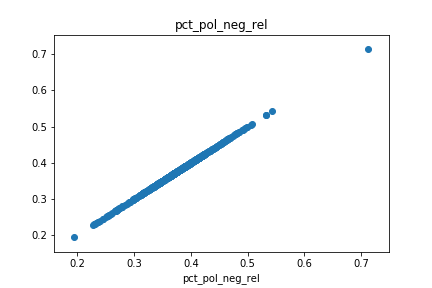
\includegraphics{00_pct_pol_neg_rel}
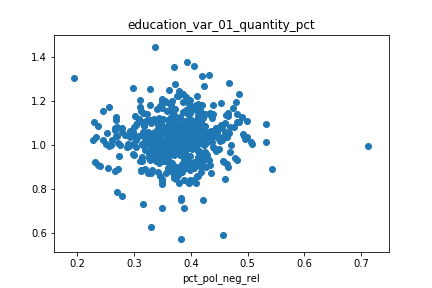
\includegraphics{01_education_var_01_quantity_pct}
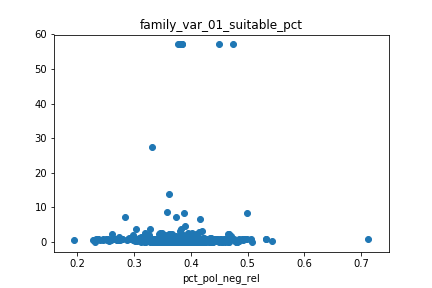
\includegraphics{02_family_var_01_suitable_pct}
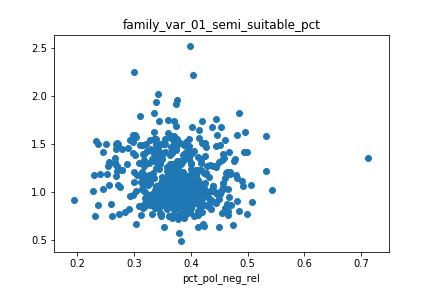
\includegraphics{03_family_var_01_semi_suitable_pct}
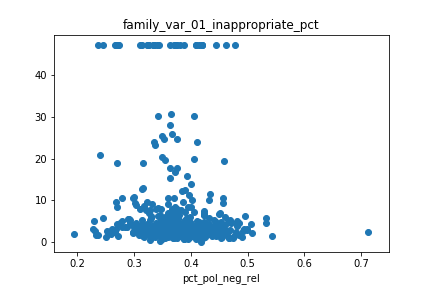
\includegraphics{04_family_var_01_inappropriate_pct}
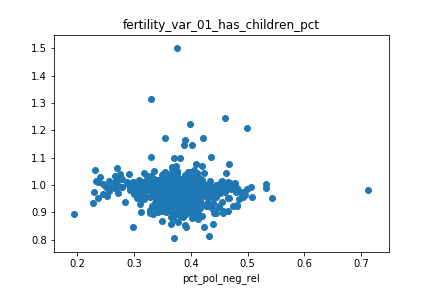
\includegraphics{05_fertility_var_01_has_children_pct}
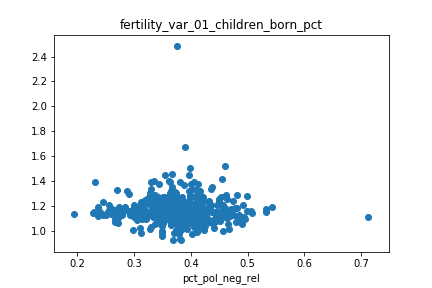
\includegraphics{06_fertility_var_01_children_born_pct}
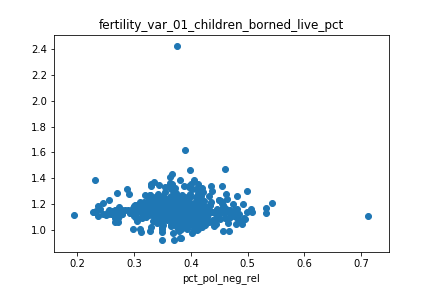
\includegraphics{07_fertility_var_01_children_borned_live_pct}
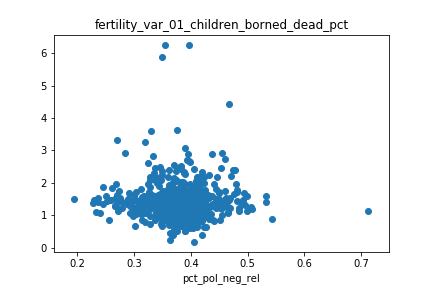
\includegraphics{08_fertility_var_01_children_borned_dead_pct}
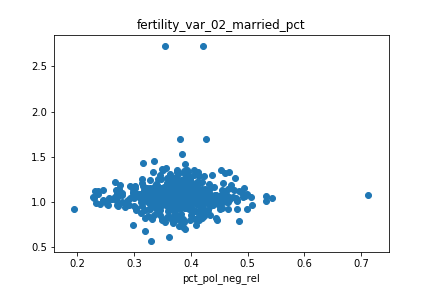
\includegraphics{09_fertility_var_02_married_pct}
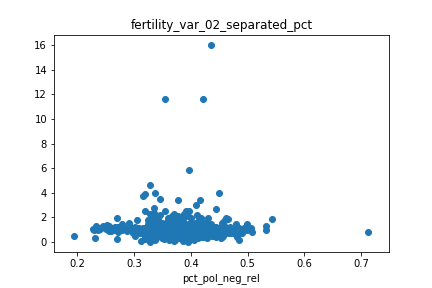
\includegraphics{10_fertility_var_02_separated_pct}
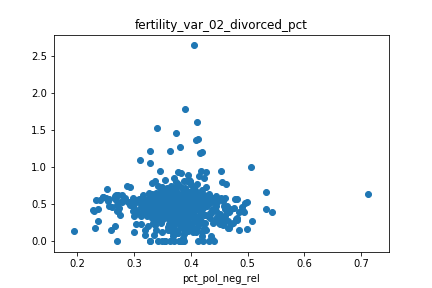
\includegraphics{11_fertility_var_02_divorced_pct}
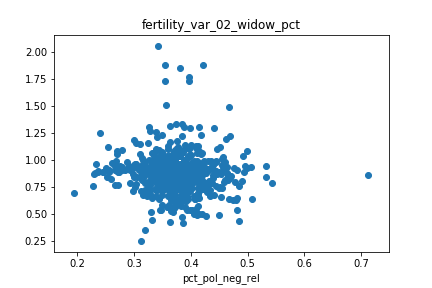
\includegraphics{12_fertility_var_02_widow_pct}
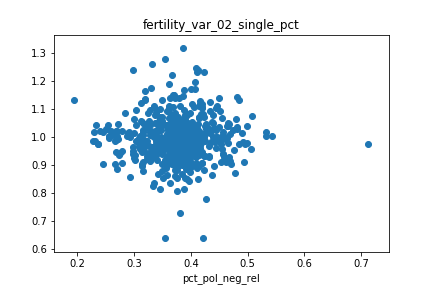
\includegraphics{13_fertility_var_02_single_pct}
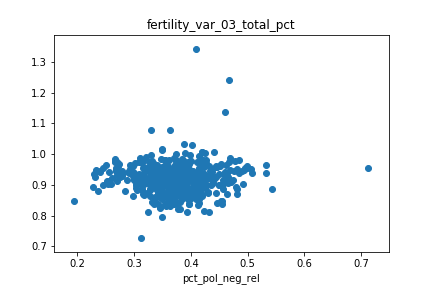
\includegraphics{14_fertility_var_03_total_pct}
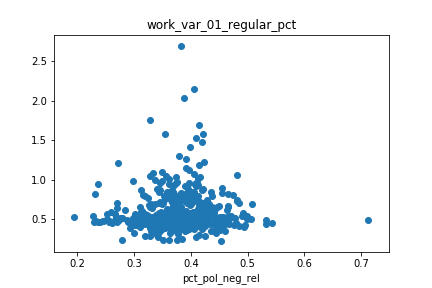
\includegraphics{15_work_var_01_regular_pct}
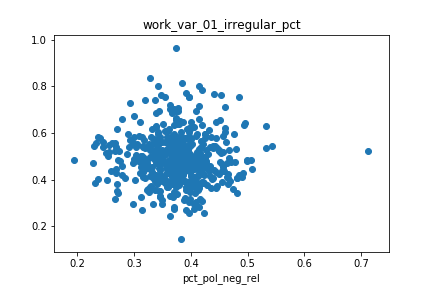
\includegraphics{16_work_var_01_irregular_pct}
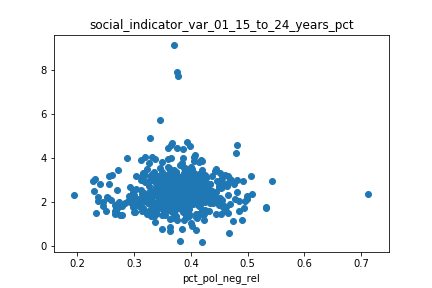
\includegraphics{17_social_indicator_var_01_15_to_24_years_pct}
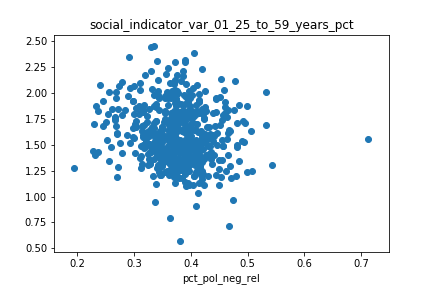
\includegraphics{18_social_indicator_var_01_25_to_59_years_pct}
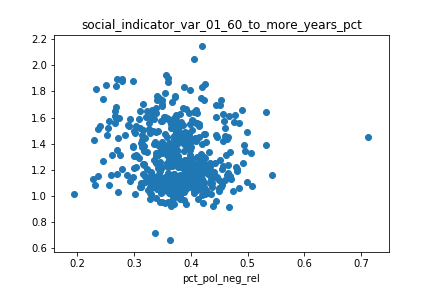
\includegraphics{19_social_indicator_var_01_60_to_more_years_pct}
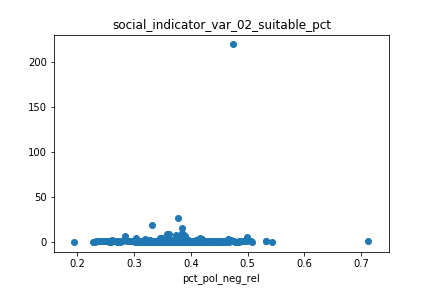
\includegraphics{20_social_indicator_var_02_suitable_pct}
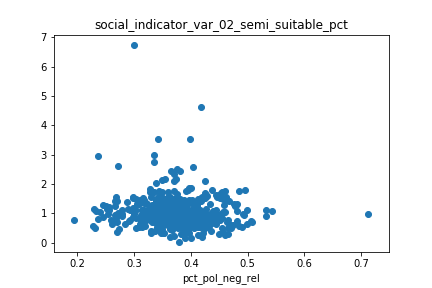
\includegraphics{21_social_indicator_var_02_semi_suitable_pct}
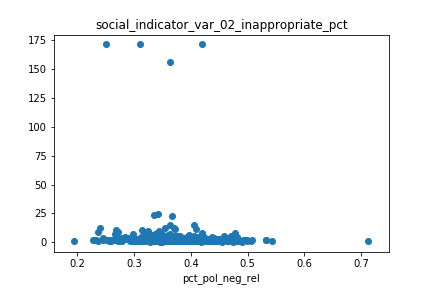
\includegraphics{22_social_indicator_var_02_inappropriate_pct}
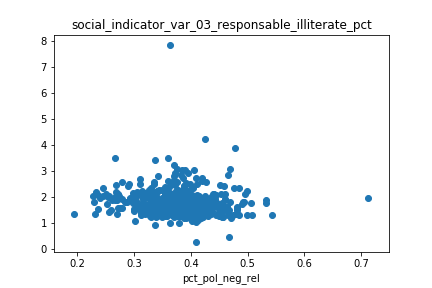
\includegraphics{23_social_indicator_var_03_responsable_illiterate_pct}
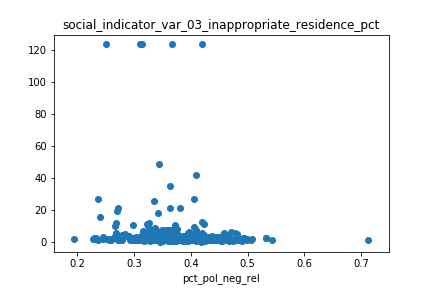
\includegraphics{24_social_indicator_var_03_inappropriate_residence_pct}
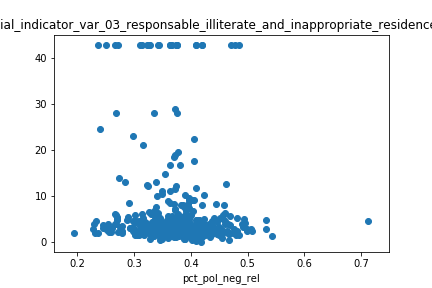
\includegraphics{25_social_indicator_var_03_responsable_illiterate_and_inappropriate_residence_pct}
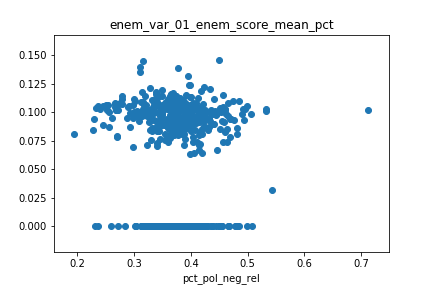
\includegraphics{26_enem_var_01_enem_score_mean_pct}
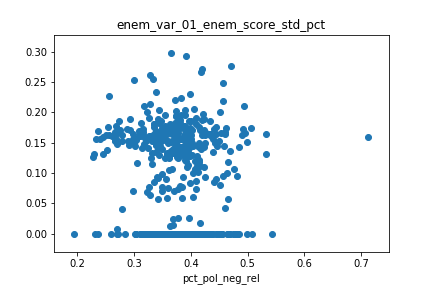
\includegraphics{27_enem_var_01_enem_score_std_pct}
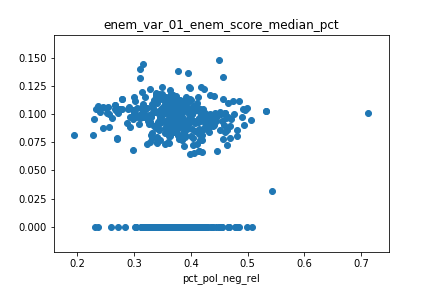
\includegraphics{28_enem_var_01_enem_score_median_pct}
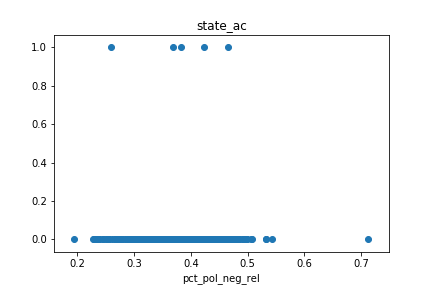
\includegraphics{29_state_ac}
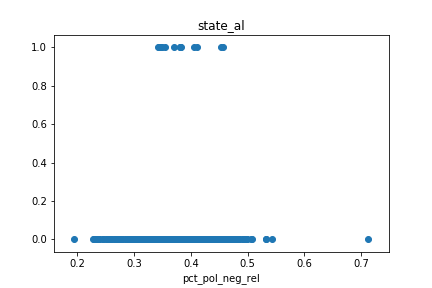
\includegraphics{30_state_al}
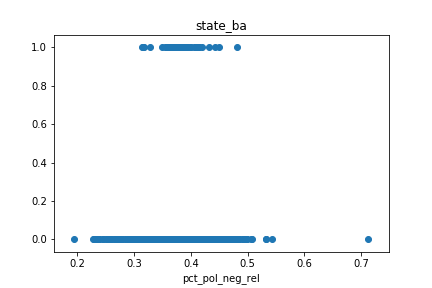
\includegraphics{31_state_ba}
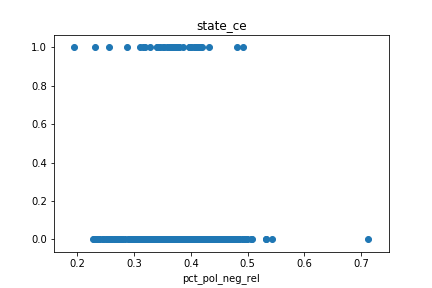
\includegraphics{32_state_ce}
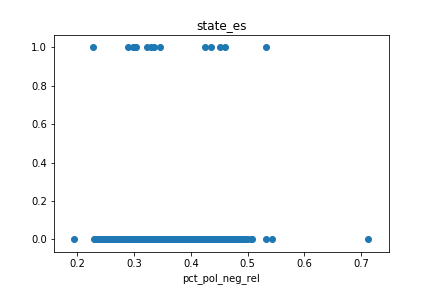
\includegraphics{33_state_es}
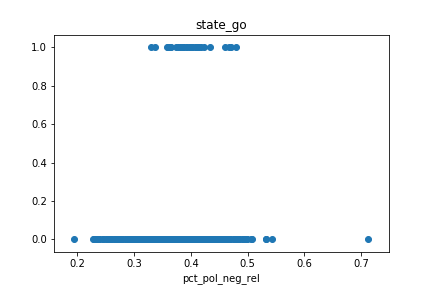
\includegraphics{34_state_go}
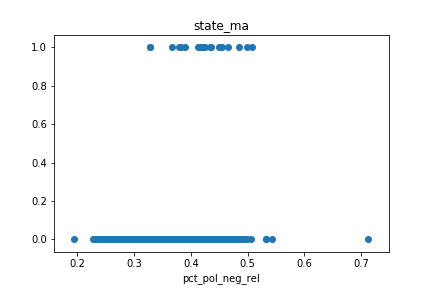
\includegraphics{35_state_ma}
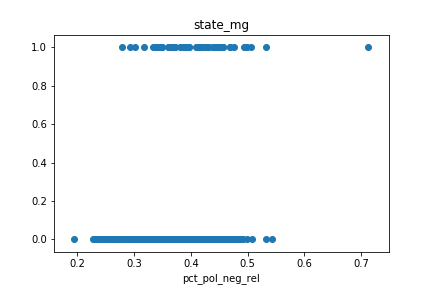
\includegraphics{36_state_mg}
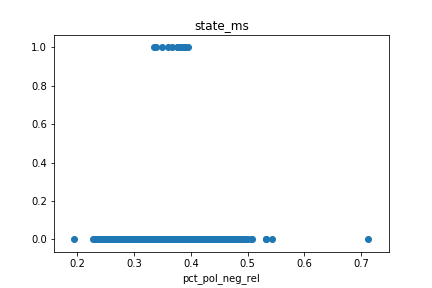
\includegraphics{37_state_ms}
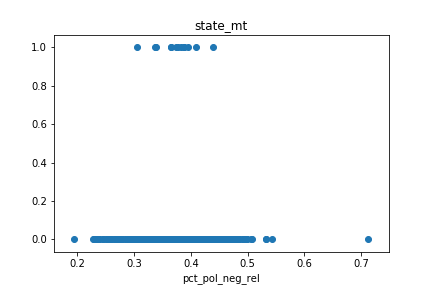
\includegraphics{38_state_mt}
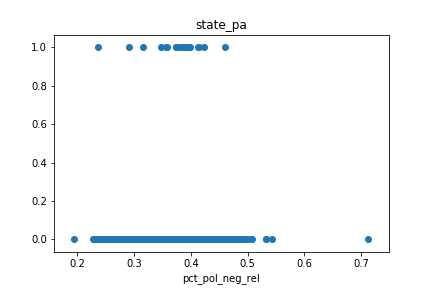
\includegraphics{39_state_pa}
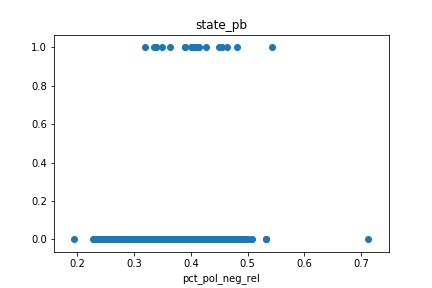
\includegraphics{40_state_pb}
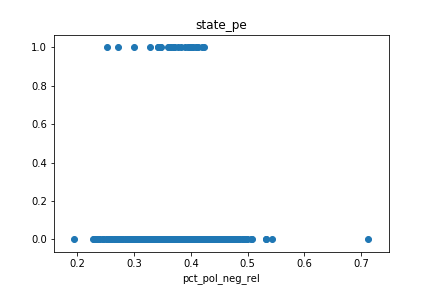
\includegraphics{41_state_pe}
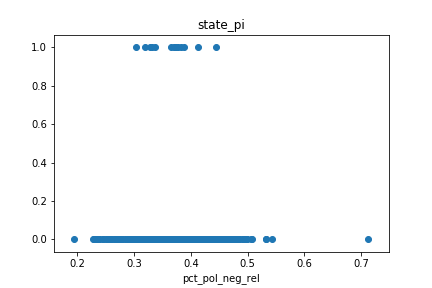
\includegraphics{42_state_pi}
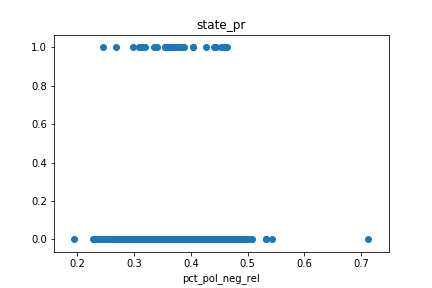
\includegraphics{43_state_pr}
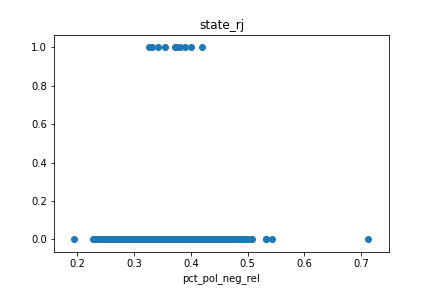
\includegraphics{44_state_rj}
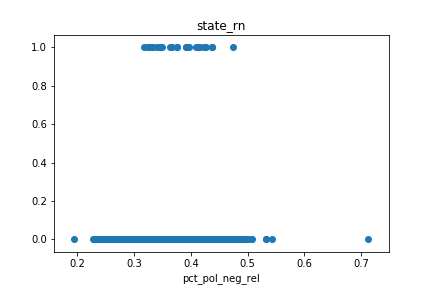
\includegraphics{45_state_rn}
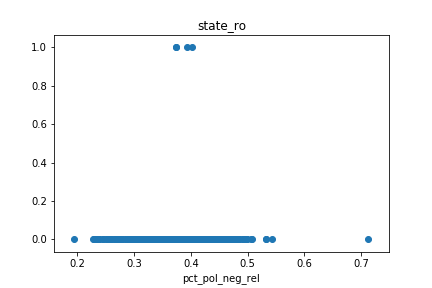
\includegraphics{46_state_ro}
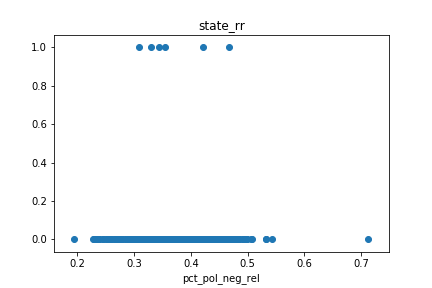
\includegraphics{47_state_rr}
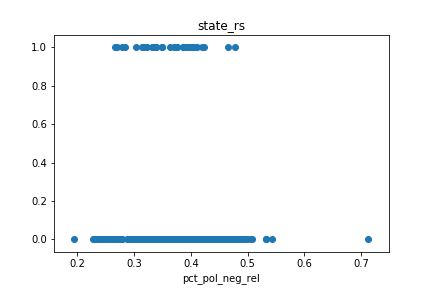
\includegraphics{48_state_rs}
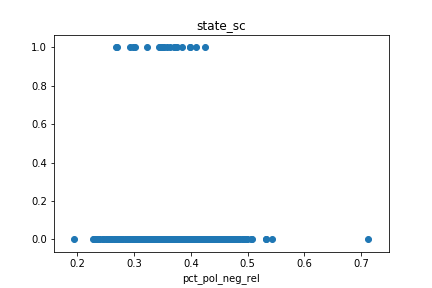
\includegraphics{49_state_sc}
\includegraphics{50_state_se}
\includegraphics{51_state_sp}
\includegraphics{52_state_to}


\graphicspath{ {./figuras/model_performance/} }
\center
\includegraphics[width=12.0cm, keepaspectratio]{cap3_scatter_reg_lin}

\captionof{figure}{Gráfico de dispersão da Regressão Linear}

\label{ape:cap3_scatter_reg_lin}



\label{ape:cap3_shap_random_forest}

\graphicspath{ {./figuras/model_performance/} }
\includegraphics{cap3_shap_random_forest}


\graphicspath{ {./figuras/model_performance/} }

\includegraphics[width=12.0cm, keepaspectratio]{cap3_scatter_random_forest}

\captionof{figure}{Gráfico de dispersão do Random Forest}

\label{ape:cap3_scatter_random_forest}



\label{ape:cap3_shap_xgboost}

\graphicspath{ {./figuras/model_performance/} }
\includegraphics{cap3_shap_xgboost}


\graphicspath{ {./figuras/model_performance/} }
\center
\includegraphics[width=12.0cm, keepaspectratio]{cap3_scatter_xgboost}

\captionof{figure}{Gráfico de dispersão do Xgboost}

\label{ape:cap3_scatter_xgboost}


% ------------------------------------------------------------------- %
% Bibliografia
\backmatter \singlespacing   % espaçamento simples
\bibliographystyle{plainnat-ime} % citação bibliográfica textual
\bibliography{bibliografia}  % associado ao arquivo: 'bibliografia.bib'

\end{document}
